\documentclass[]{article}
\usepackage{amsthm}
\usepackage{amsmath}
\usepackage{amssymb}
\usepackage{mathrsfs}
\usepackage{amssymb,amsfonts}
\usepackage{enumerate}
\usepackage{mathrsfs}
\usepackage{extarrows}
\usepackage{mathtools}
\usepackage{hyperref}
\usepackage{MnSymbol}

\usepackage{pifont}
\newcommand{\cmark}{\ding{51}}
\newcommand{\xmark}{\ding{55}}
\def\ZZb{\mathbb{Z}_2}
\def\ZZ{\mathbb{Z}}
\def\Soc{\rm soc}
\def\FF{\mathbb F}
\def\CC{\mathbb C}
\def\RR{\mathbb R}
\def\NN{\mathbb N}
\def\curlyB{\mathscr B}
\def\CL{\mathcal{L}}

\newcommand{\bmat}[4]{\begin{bmatrix} #1 & #2 \\ #3 & #4\end{bmatrix}}


\usepackage[svgnames]{xcolor}
\usepackage{tikz}
\usepackage{float}
\usepackage{cutwin}
\usetikzlibrary{arrows}
\usetikzlibrary{graphs}
\usetikzlibrary{graphs.standard}
\usetikzlibrary{decorations.markings}

\pgfdeclarelayer{edgelayer}
\pgfdeclarelayer{nodelayer}
\pgfsetlayers{edgelayer,nodelayer,main}

\tikzstyle{none}=[inner sep=0pt]


\newlength{\imagewidth}
\newlength{\imagescale}

%theoremstyle{plain} --- default
\newtheorem{thm}{Theorem}[section]
\newtheorem*{thm*}{Theorem}
\newtheorem*{cor}{Corollary}
\newtheorem{prop}[thm]{Proposition}
\newtheorem*{prop*}{Proposition}
\newtheorem*{clm}{Claim}
\newtheorem{lem}[thm]{Lemma}
\newtheorem{conj}[thm]{Conjecture}
\newtheorem*{quest}{Question}

\theoremstyle{definition}
\newtheorem*{defn}{Definition}
\newtheorem*{defns}{Definitions}
\newtheorem{con}[thm]{Construction}
\newtheorem*{exmp}{Example}
\newtheorem*{exmps}{Examples}
\newtheorem{notn}[thm]{Notation}
\newtheorem{notns}[thm]{Notations}
\newtheorem{addm}[thm]{Addendum}
\newtheorem{exer}[thm]{Exercise}

\theoremstyle{remark}
\newtheorem*{rem}{Remark}
\newtheorem*{rems}{Remarks}
\newtheorem{warn}{Warning}
\newtheorem{sch}{Scholium}




\makeatletter
\let\c@equation\c@thm
\makeatother
\numberwithin{equation}{section}

\bibliographystyle{plain}

%--------Meta Data: Fill in your info------
\title{M3/4 P55 Algebraic combinatorics}

\date{Spring 2015}
\author{Lectured by: Martin Liebeck}
\begin{document}

\maketitle

\tableofcontents

\setcounter{section}{-1}
\newpage
\section{Introduction}
	\begin{itemize}
		\item Combinatorics is a study of discrete structures.
		\item in the scope of this course we will deal with:
		\begin{itemize}
			\item Codes
				\begin{itemize}
				\item Subsets of $\ZZb^n$ where $\ZZb = \{0,1\}$
				\end{itemize}
			\item Graphs
				\begin{itemize}
				\item sets of vertices with edges connecting them. Essentailly a set with a collection of pairs. They can also be represented as adjacency matrices
				\end{itemize}
			\item Designs
				\begin{itemize}
					\item Originated in statistical theory of experiments
					\item Collections of subsets of agiven set
				\end{itemize}
		\end{itemize}
		\item We will use tools from linear algebra to study those discrete structurs.
		\item \url{http://wwwf.imperial.ac.uk/~mwl/m3p17/}
	\end{itemize}

	\subsection{Codes}
		Everyday language consists of an alphabet and words which are distinguished admissible strings of letters. For a machine language the alphabet is going to consist of:
		\begin{itemize}
			\item alphabet = $\{0,1\}$
			\item some admissible combinations of those letters (strings) e.g. $001010$, we are going to call these codewords
		\end{itemize}
		Eg. ASCII code for keyboard symbols maps each letter to 0s and 1s, 7bit words (binary strings 7 letters long)
		\begin{itemize}
			\item A corresponds to $01000001$
			\item B corresponds to $01000010$
		\end{itemize}

		And so on

		\begin{exmp}\hfill\\
		Message: Liebeck has £10000\\
		encoded into ASCII codewords:\\
		\[
		L \rightarrow 01001100
		\]
		etc.\\

		Transmitted over a digital medium.\\
		\\
		Then receiver takes the string of binary codewords and decodes it using the ASCII map, giving back the original message: “Liebeck has £1000”\\
		\\
		Suppose the bank has refused the message. Errors can occur at transceiver stage on average in 1 in 1000 bits (for example)
\\
		\\
		Different kinds of errors can occur (replace 1 with 0, lose a bit of information or cut off)
\\
		\\
		This calls for error correction schemes. Ordinary language has a lot of redundancies, i.e. words can easily be corrected \\
		\\
		E.g. \emph{Algubreic Cumbinatorocs} can easily be corrected, because there are not many similar words in the English language, and there is a set of admissible words in English, not every combination of letters is a word.\\
		\\
		Machine language should have a similar correction scheme - part of the theory of machine languages is to build in some redundancy into the language\\
		\end{exmp}

		\begin{exmp}\hfill\\
		E.g. Yes/No code:\\
		message is 1 or 0\\
		\\
		Sending just one or zero is not sufficient, because you could send a wrong digit and get the wrong answer\\

		one example of such redundant code would be to map the words the following way:
\\
			\begin{align*}
				\text{yes} &\rightarrow 111\\
				\text{no} &\rightarrow 000\\
			\end{align*}
		If a single error is made, e.g. we send 011 instead of 111 we can correct it
		\end{exmp}
		This is called an error correcting code, and this code corrects 1 error\\
		\\
		Suppose we want to send messages in a larger language, consisting of more than 2 messages.\\
		\begin{exmp}
			This code will be able to send 8 messages and correct 1 error (the code contains 8 codewords)\\
			\\
			Messages: $abc$ in $\ZZb$\\
			Codewords:\\
			\begin{align*}
				&abcxyz \qquad (a,b,c \in ZZ_2) \text{and $xyz$ depend on $abc$}\\
				&x = a+b\\
				&y = b+c\\
				&z = a+c\\
			\end{align*}
			$C = \{000 000, 100 101, … , 111 000\}$\\
			Suppose we receive $011 110$:\\
			Well:\\
			\begin{align*}
				a + b &= 1 &= x\\
				b + c &= 0 &\neq y\\
				a + c &= 1 &\neq z = 0\\
			\end{align*}
			So there is an error. Where is it? Well it is in $c$ because it breaks the $y$ and $z$ checksums\\
			So the corrected codeword is $010 110$\\
			\\
			Claim:\\
			This code can correct 1 error\\
			\begin{table}[h]
			\begin{tabular}{lllllll}
			Error in: & \multicolumn{1}{l|}{a} & \multicolumn{1}{l|}{b} & \multicolumn{1}{l|}{c} & \multicolumn{1}{l|}{x} & \multicolumn{1}{l|}{y} & \multicolumn{1}{l|}{z} \\ \hline
			$x=a+b$   & \xmark & \xmark & \cmark & \xmark & \cmark & \cmark  \\
			$y=a+c$   & \cmark & \xmark & \xmark & \cmark & \xmark & \cmark  \\
			$z=a+c$   & \xmark & \cmark & \xmark & \xmark & \cmark & \cmark
			\end{tabular}
			\end{table}
			So pattern of \cmark and \xmark determines the eror
		\end{exmp}
		The aim of coding theory: Find codes $C $ s.t:\\
		\begin{itemize}
			\item $C$ has lots of codewords
			\item $C$ corrects “enough” errors
			\item We don’t want the codewords to be “too long”
		\end{itemize}
	\subsection{Graphs}
		A \emph{graph} is a pair $(V, E)$ where $V$ is the set of \emph{vertices} and $E$ is a collection of pairs: $\{\{x,y\}: x,y \in V\}$ called \emph{edges}\\
		\\
		E.g. $V = \{1,2,3,4\}, \qquad E = \{\{1,2\}, \{1,3\}, \{2,4\}, \{2,3\}\}$\\

		\begin{tikzpicture}
			\graph [simple] {
			subgraph K_n [n=4, clockwise];
			1 -!- 4;
			3 -!- 4;
			};
		\end{tikzpicture}

		We will study a special type of graphs that can be expressed as codes and lend themselves well to algebraic methods\\
		\begin{defn}
		For a \emph{vertex} $x$, call the other vertices connected to $x$ by an \emph{edge} \emph{``neighbours''}
		\end{defn}

		\begin{defn}
		We call the graph $\Gamma$ \emph{regular} if every vertex has the same number of neighbours, say $K$. This number $K$ is called the \emph{valency} of the graph
		\end{defn}
		E.g. any polygon is a regular graph with a valency = 2\\
		\\
		\begin{figure}[H]
			\begin{tikzpicture}
				\graph [simple] {
					subgraph C_n [n=4, clockwise];
				};
			\end{tikzpicture}
			\begin{tikzpicture}
				\graph [simple] {
					subgraph C_n [n=3, clockwise];
				};
			\end{tikzpicture}
			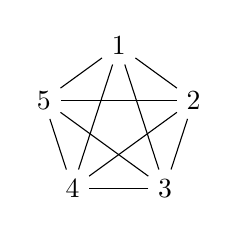
\begin{tikzpicture}
				\graph [simple] {
					subgraph K_n [n=5, clockwise];
				};
			\end{tikzpicture}
		\end{figure}
		\begin{defn}

		A graph $\Gamma$ is \emph{strongly regular} if:
		\begin{enumerate}
			\item $\Gamma$ is regular, valency $K$
			\item Any pair of joined vertices has the same number a of common neighbours
			\item Any pair of non-joined vertices has the same number b of common neighbours
		\end{enumerate}
		\end{defn}
		\emph{Petersen graph} is a strongly regular graph of valency 3\\

		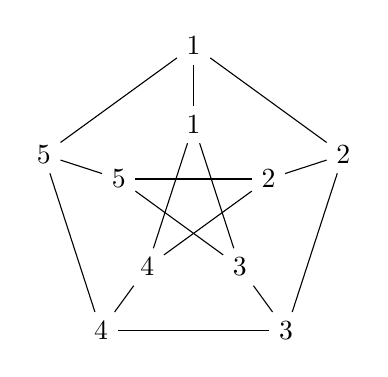
\begin{tikzpicture}
		  \graph [clockwise] {
		     subgraph C_n [n=5,name=A, radius=2cm];
		     subgraph I_n [n=5,name=B, radius=1cm];
		     \foreach \i [evaluate={\j=int(mod(\i+2,5)+1);}] in {1,...,5}{
		        A \i -- B \i;
		        B \i -- B \j;
		     }
		  };
		\end{tikzpicture}
		\begin{thm}[Kuratowski, 1930]\hfill\\
		A graph $G$ is planar iff $G$ does not contain a subdivision of $K_5$ or $K_{3,3}$
		\end{thm}
		\begin{proof}\hfill\\
		A Kuratowski subgraph of $G$ is a subgraph of $G$ that is a subdivision of $K_5$ or $K_{3,3}$ . A minimal nonplanar graph is a nonplanar graph such that every proper subgraph is planar.
		\end{proof}

		\begin{thm}[Friendship Theorem, Erdös, Remyi]\hfill\\
		In a community where any two people have exactly one common acquaintance, there is someone who knows everyone.
		\end{thm}
		This can be described as a graph:\\
		\\
		Vertices are the people and we join the people with edges representing the “know each other” relation\\
		\\
		The condition from the theorem is that they have one shared acquaintance, i.e. any two vertices have exactly one common neighbour\\
		\\
		We want to show that there exists a vertex that is connected to all of the other vertices in the graph\\
		\\
		\begin{tikzpicture}
			\graph [simple] {
				subgraph C_n [n=4, clockwise] -> 5;
				1 -!- 4;
				2 -!- 3;
			};

		\end{tikzpicture}
		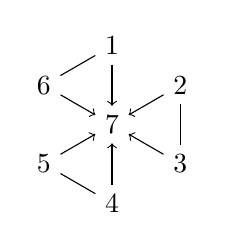
\begin{tikzpicture}
			\graph [simple] {
				subgraph C_n [n=6, clockwise] -> 7;
				1 -!- 2;
				3 -!- 4;
				5 -!- 6;
			};
		\end{tikzpicture}
		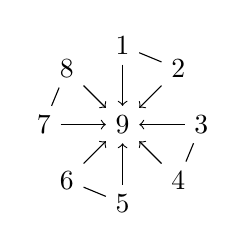
\begin{tikzpicture}
			\graph [simple] {
				subgraph C_n [n=8, clockwise] -> 9;
				1 -!- 8;
				2 -!- 3;
				4 -!- 5;
				6 -!- 7;
			};
		\end{tikzpicture}
		\\
		All the known proofs use linear algebra - matrix representations of graphs become incredibly useful/powerful\\
	\subsection{Designs}
		Used in statistics and experimental design.\\
		\\
		Suppose we have v varieties of a product (say chocolate) to be tested by concumers.\\
		We want:\\
		\begin{enumerate}
			\item each consumer to test $k$ varieties
			\item each variety tested by some no. $r$ of consumers
		\end{enumerate}

		\begin{exmp}\hfill\\
			Eg. $v =9, k = 4, r =3$\\
			No of consumers must be $b = \frac{vr}{k} = 6$\\
			\\
			consumers $c_1, …, c_6$ testing:\\
			\begin{table}[h]
				\begin{tabular}{llllll}
				$c_1$  & $c_2$  & $c_3$  & $c_4$  & $c_5$  & $c_6$ \\
				$1234$ & $5678$ & $1357$ & $2468$ & $1247$ & $3568$ \\
				\end{tabular}
			\end{table}
		\end{exmp}
		\begin{defn}\hfill\\
		Let $X$ be a set, $v = |X|$ and let $\mathscr{B}$ be a collection of subsets of $X$.\\
		Call $(X, \mathscr{B})$ (or just $\mathscr{B}$) a \emph{design} if:\\
		\begin{enumerate}
			\item every set in $\mathscr{B}$ has size $k$
			\item every element of $X$ lies in $r$ subsets of $\mathscr{B}$
		\end{enumerate}
		\end{defn}
		The subsets in $\mathscr{B}$ are called the \emph{blocks} of design.\\
		Pareamters are $(v,k,r)$\\
		Example above is $(8,4,3)$\\
		\\
		Interesting condition: each pair of varieties is tested by the same number of consumers.\\
		\\
		\begin{defn}
		A design $(X, \mathscr{B}$) is a \emph{2-design} if any two points (elements of $X$) lie in the same number of blocks.

		The larger t is, the stronger this condition is.

		For large t, nontrivial t-designs are rather rare.
		(e.g. the first nontrivial 6-design was found in 1980’s).
		\end{defn}
		Example: $(8,4,3)$ is not a 2-design\\
		\\
		In general for $t \geq 1$ say $\mathscr{B}$ is a t-design if any $t$ points lie in the same number of blocks.\\
		The larger $t$ is, the stronger this condition is.\\
		For large $t$, nontrivial t-designs are rather rare. (e.g. the first nontrivial 6-design was found in 1980’s).\\
		\\
		For $t = 2$ there is a lot of nice theory, links to coding theory \& graph theory included in the course. They also lend themselves nicely to examples:\\
		\\
		\begin{exmp}[A nice example of 2 design]\hfill\\
		(Idea: take any two points in a plane, you can draw a line through them)\\
		Replace $\RR^2$ by a finite field, for example $\ZZ_p^2$\\
		Let $p$ be a prime, recall:
\\
		\[
			\ZZ_p = \text{integers up to p-1}
		\]
		with addition and multiplication mod p (ring structure) - making it a field (group under addition $\ZZ_p\setminus\{0\}$ a group under multiplication, plus obeys distributive laws).\\

		Now let $\ZZ_p^2 = \text{vectors with coordinates in $\ZZ_p$}$\\
		Call it the \emph{affine plane} over $\ZZ_p$\\
		\\
		Define a line in $\ZZ_p^2$ to be a subset of the form  $\{a + \lambda b: \lambda \in \ZZ_p\}$
		where $(a,b)$ are fixedvectors in $\ZZ_p^2$

		Fact (exercise) any two vecros in $\ZZ_p^2$ are in a unique line
		Now define:
		\begin{align*}
			X &= \ZZ_p^2\\
			\text{Blocks}\; &= \;\text{collection of lines}
		\end{align*}
		 Then this is a 2-design with parameters: $(p^2, p, p+1)$ (convince yourself it’s not $p$) where any 2 points lie in exactly 1 block (they are tested against each other once)\\
		\end{exmp}

\newpage
\section{Error correcting codes}
	Define $\ZZb = {0,1}$ with addition and multiplication modulo 2\\
	\\
	and $\ZZb^n = \{(x_1,…, x_n): x_i \in \ZZb\}$ (often we will drop brackets and commas)\\ with the usual addition and scalar multiplication of vectors.\\
	$\ZZb^n$ is vector spaces over $\ZZ_2$ with standard basis $e_1, …,e_n (e_i = 0,…1,…0)$ (1 in ith place) and dimension $n$.

	\begin{defn}
		 A code $C$ of length $n$ is a subset of $\ZZ_2^n$. The vectors in $C$ are called \emph{codewords}.
	\end{defn}
	% numbering here?
	\begin{defn}
		Distance between two vectors in $\ZZ_2^n$ is:\\
		$d(x,y) = \sum_i x_i - y_i$ (number of places where they are different)

	\end{defn}
	Claim this is a metric on $\ZZ_2^n$, (i.e. it satisfies the triangle inequality)
	\begin{prop}[Triangle inequality]\hfill\\
	$d(x,y) + d(x,z) \geq d(x,z)$
	\end{prop}
	\begin{proof}\hfill \\
	Let:\\
	\begin{align*}
		A &= \{i: x_i \neq{!=}z_i\}\\
		B &= \{i: x_i = y_i, x_i \neq{!=} z_i\}	\\
		C &= \{i: x_i \neq{!=} y_i, x_i \neq{!=} z_i\}\\
	\end{align*}
	So $C$ is the compliment of $B$ in $A$\\
	So |$A| = |B| + |C|, d(x,z) = |A|$\\
	and since $d(x,y) \geq |C|$ and $d(y,z) \geq|B|$ we get the triangle inequality
	\end{proof}

	\begin{defn}\hfill\\
	Let $C \subseteq \ZZ_2^N$ be a code\\
	The minimum distance $d(C)$ of $C$ is:\\
	\[
		d(C) = min \{ d(x,y): x,y \in C, x \neq y\}
	\]
	\end{defn}

	\subsection{Error correction}
		Let $C$ in $\ZZ_2^n$ and $e\in \NN$.
		Suppose a codeword $c \in C$ is sent and at most $e$ errors are made.\\
		Additionally, suppose a vector $v$ is received.\\
		Then we say $C$ corrects $e$ errors if the closest codeword to $v$ is $c$.\\
		\begin{defn}\hfill\\
		$C \in \ZZ_2^n$ corrects $e$ errors if for any $c_1, c_2 \in C$ and $w \in \ZZ_2^n$:\\
		\[
			d(c_1,w) \leq e, d(c_2, w) \leq e\quad \Rightarrow \quad c_1 = c_2
		\]%check here

		Equivalent definition:\\
		\\
		For $c \in C$ define sphere $S_l(c) = {w \in \ZZ_2^n: d(c,w) \leq l}$\\
		Then $C$ corrects $e$ errors if for all $c1, c_2 \in C, \quad c_1\neq2 $:\\
		\[
			S_e(c_1) \cap S_e(c_2) \neq \emptyset
		\]

		\end{defn}
		\begin{prop}\hfill \\
		Code $C$ corrects $e$ errors $\Leftrightarrow \quad d(C) \geq 2e+1$
		\end{prop}
		\begin{proof}\hfill\\
		$(\Rightarrow)$ Excercise sheet\\
		$(\Leftarrow)$: \\
		Suppose $d(C) \geq 2e+1$\\
		Let $c_1, c_2 \in C $ and suppose $w \in \ZZ_2$ satisfies $d(c_1, w) \leq e, d(c_2,w) \leq e$\\
		\\
	 	Then by the triangle inequality\\
	 	\begin{align*}
		d(c_1,c_2) &\leq d(c_1,w) + d(c_2, w)\\
		d(c_1,c_2) &\leq 2e\\
		\end{align*}
		but $d(C) \geq 2e +1$\\
		so $C$ corrects $e$ errors and $c1 = c2$\\
		\end{proof}
	\subsection{Linear codes}
		\begin{defn}\hfill\\
			A linear code is a code $C$ which is a subspace of $\ZZ_2^n$\\
		\end{defn}
		I.e:\\
		\begin{enumerate}
			\item $0 \in C$
			\item $x,y \in C \Rightarrow x+y \in C$ (subgroup group under addition)
		\end{enumerate}
		Basic construction of codes using matrices:
		\begin{prop}
			Let $A$ be an $m \times n$ matrix over $\ZZ_2$\\
			then $C = {x \in \ZZ_2^n\quad:\quad Ax = 0}
$ is a linear code and $dim C = n - rank(A)
$
		\end{prop}
		E.g:\\
		\begin{align*}
			C_3 &= \left\{abcxyz \in \ZZ_2^6\quad :\quad x = a +b, y + b+c, z = a +c \right\}\\
	       &= \left\{ x \in \ZZ_2^6\quad :\quad \left(\begin{smallmatrix}
	       			1&1&0&1&0&0\\
	       			0&1&1&0&1&0\\
	       			1&0&1&0&0&1\\
	       		\end{smallmatrix}\right) x = 0\right\}
		\end{align*}
		is a linear code of dimension 3 with basis $100101,\ 010110,\ 001011$

		\begin{prop}\hfill\\
			If $C$ is a linear code of dimension $k$, then the number of codewords :$|C| = 2^k$
		\end{prop}
		\begin{proof}\hfill''
		 Let $c_1, ..., c_k$ be a basis of $C$\\
		 \\
		Every $c \in C$ is a unique linear combination of the basis elements:\\
			\[
			c = \lambda_1 c_1 + ... + \lambda_k c_k \qquad \lambda_i \in \ZZ_2
			\]

		There are 2 choices for each $\lambda_i$, giving $2^k$ choices for $\sum_{i=0}^k\lambda_i c_i$ giving $2^k$ codewords.
		\end{proof}
	\subsection{Minimum Distance}
		\begin{defn}
			For $x \in \ZZ_2^n$, the weight of $x$ is $wt(x) = \text{no of coords of x equal to 1}$
		\end{defn}
		Observe:\\
		$wt(x) = d(x, 0)$ and $wt(x+y) = d(x,y)$, as $x+y$ has a $1$ precisely at the coords where $x$ and $y$ differ\\
		\\
		\begin{prop}\hfill\\
		Let $C$ be a linear code, then minimum distance $d(C)$ between codewords is:\\
		\[
			d(C) = \text{min} \{ wt(c)\quad:\quad 0 \neq c \in C\}
		\]
		\end{prop}
		\begin{proof}\hfill\\
		Let $c \in C, c \neq 0$ have minimal weight say $wt(c) = r$\\
		As $C$ is linear, $0 \in C$, and $d(c,0) = wt(c) = r$\\
		Therefore we have found two codewords, $r$ apart\\
		So $d(C) \leq r$\\
		\\
		Now let $x,y$ be codewords in $C x,y\quad \neq \quad 0, x\quad \neq \quad y$\\
		\\
		Then $x+y \in C$ and so \\
		\\
		\[
			wt(x+y)\geq r
		\]
		Hence $d(x,y) = wt(x+y) \geq r$ \\
		So $d(C) \geq r$ Therefore $d(C) = r$\\
		\end{proof}
		Example:
		Code $C_3 \in \ZZ_2^6$\\
		Check that min $\{wt(c) \quad:\quad 0 \neq c \in C_3\} = 3$\\
		Hence $d(C_3) = 3$ so $C_3$ corrects 1 error by prop 1.2\\
		\\

		Aims:\\
		Find linear codes $C \in \ZZ_2^n$ s.t:\\
		\begin{itemize}
		\item $dimC$ is large
		\item $d(C)$ is large
		\item length is small
		\end{itemize}

		Matrix algebra will provide us with nice tools to achieve that.
	\subsection{Check matrix}

		\begin{defn}
		Suppose \(A\) is a \(m \times n\) matrix over \(\ZZb\) and:
		\begin{equation*}
		C = \{ x \in \ZZb^n : Ax = 0\}
		\end{equation*}
		We call A a check matrix of the linear code $C$
		\end{defn}

		\begin{prop}
		Suppose the check matrix $A$ of a linear code $C$ satisfies

		\begin{enumerate}
			\item $A$ has no $0$ column
			\item $A$ has no two equal columns
		\end{enumerate}
		Then $C$ corrects 1 error.
		\end{prop}

		\begin{proof}
		Suppose false. Then $d(C) \leq 2$ by proposition 1.2.
		Hence by propsoition 1.5 $\exists 0\neq c \in C$ s.t $wt(C) = 1 || 2$

		Suppose $wt(c) = 1$. Then $c = e_i = (0 ... 1 ...)$ and

		$A_C = 0 \implies Al_i = 0 \implies \text{ith col of $A$} = 0$ Contradiction

		Suppose $wt(c) = 2$ then $c = e_i + e_j$ so
		$Ac = 0 \implies Al_u + Al_j = 0 \implies ith col of A = jth col of A$ contradiction
		\end{proof}

		Examples

		\begin{enumerate}
		\item
		\[C_3 = \{
			x \in \ZZb^6 : \begin{bmatrix}
			1 & 1 & 0 & 1 & 0 & 0 \\
			0 & 1 & 1 & 0 & 0 & 0 \\
			1 & 0 & 1 & 0 & 0 & 1
			\end{bmatrix}x = 0
		\}\]
		Corrects 1 error by 1.6

		\item Suppose we want a code $C$ which corrects 1 error and has $3 \times n$ check matrix for some n. What is max dim of $C$?
		Answer:
		By 1.6 need to find largest n s.t. $\exists 3 \times n $ check matrix with distinct non zero cols (in$\ZZb^3$). Such a matrix will have as cols all non zero vectors in $\ZZb^3$ of which there a re 7, eg:

		\[
		A = \begin{bmatrix}
			1 & 1 & 1 & 0 & 1 & 0 & 0 \\
			1 & 1 & 0 & 1 & 0 & 1 & 0 \\
			1 & 0 & 1 & 1 & 0 & 0 & 1
			\end{bmatrix}
		\]

		this is a $3\times 7$ so in check matrix of code $C$ of length 7 dim 4 (by rank nullity) correcting 1 error.

		This sends 16 messages abcd using codewords abcdxyz where
		\[
			x = a + b + c,\\
			y = a +b + d \\
			z = a + c + d
		\]
		This is called a Hamming code $\text{Ham}(3)$

		\end{enumerate}
	\subsection{Correcting an error}
		Suppose a codeword $c$ is sent and 1 error is made, so that received vector is $c'$ which is not necessarily a code. How do we correct the error?

		Well, $c' = c + l_i$ for some $i$
		So

		\begin{align*}
			Ac' &= A(c+l_i) \\
				&= A\ c + A\ l_i \\
				&= A\ l_i \\
				&= \text{$i^\text{th}$ col of $A$}
		\end{align*}

		E.g. Let $C = \text{Ham}(3)$.
		Suppose received vector is $c= (1101000)^T$.

		Then \[
			A\ c' = \left(\begin{smallmatrix}0\\1\\0\end{smallmatrix}\right) = \text{$6^\text{th}$ column of $A$}
		\]
	\subsection{Hamming Codes}

		\begin{defn}
		Let $k\geq3$ A Hamming Code Ham$(k)$ is a code fo which the check matrix has as columns all the distinct non zero vectors in $\ZZb^k$
		\end{defn}


		\begin{prop}
		\begin{enumerate}
			\item Ham$(k)$ has length $2^k-1$, dim $2^k-1 - k$
			\item Ham$(k)$ corrects 1 error
		\end{enumerate}
		\end{prop}
		\begin{proof}
			\par
			\begin{enumerate}
			\item\par
				Since there are $2^k-1$ non zero vectors in $\ZZb^k$ check matrix of Ham$(k)$ is $k\times (2^k-1)$ and rank $k$
			\item\par
				Follows from 1.6
			\end{enumerate}
		\end{proof}

		\begin{defn}
		Let $C, C' \subseteq \ZZb^n$. Say $C$ and $C'$ are equivalent codes if there is a permutation of the coordinates sending codewords in $C$ bijectively to codewords in $C'$. (This is equivalent to permuting the columns of the checkmatrices)
		\end{defn}

		E.g all Hamming codes ham$(k)$ are equivalent.

		We want codes that correct more than one error though. Ideally we would like to have a matrix condition that corrects lots of errors - we would like to generalize definition 1.6

		\begin{prop}
		Let $d \geq 2$ and let $C$ be a code wit hcheck matrix $A$.
		\begin{enumerate}
			\item\par Suppose every set of $d-1$ columns of $A$ is linearly independent. If that is true, then the minimum distance $d(C) \geq d$
			\item\par Suppose in addition to (1) that $\exists$ a set of $d$ columns of $A$ that are linerarly dependent. then $d(C) = d$
		\end{enumerate}
		\end{prop}

		\begin{proof}
		\begin{enumerate}
			\item\par Suppose false, and $d(C) \leq d-1$. Then $\exists 0 \neq c \in C$ with $wt(c) = r \leq d-1$. Write $c$ as a sum of standard basis vectors:
			\[
				c = e_{i_1} + ... + e{i_r}
			\]

			So \[
				0 = Ac = Ae_{i_1} + ... + Ae{i_r}
			\]
			\[
				= \text{col}i_1 + ... + \text{col}i_r
			\]

			This is a contradiction, since by the hypothesis of (1) any set of $r \leq d-1$ columns is linearly independent.

			\item\par
			Suppose columns $i_1 ... i_d$ are linearly dependent, say

			\[
				\lambda_1 (\text{col})i_1 + ... \lambda_d(\text{col})i_d = 0, \lambda_i \in \ZZb
			\]

			As by (1) any $d-1$ columns are linearly independent, all of $\lambda_i = 1 \forall i$. Then

			\[
				0 = \text{col}i_1 + ... \text{col}i_d
			\]

			\[
				= A(e{i_1} + ... e{i_d})
			\]

			Then $c = e{i_1} + .. + e{i_d} \in C$ and $wt(c) = d$
		\end{enumerate}
		\end{proof}

		E.g

			Find a linear code of length 9 dimension 2 which corrects 2 errors.
			Answer:
			Check matrix $A$ should be a $7 \times 9$ matrix (of rank 7).
			Also need code $C = \{x \in \ZZb^9: Ax = 0\}$ to have $d(C)\geq 5$ so by 1.8 want every set of 4 columns of $A$ to be linearly independent.

			Take
			\begin{equation*}
				A = \begin{bmatrix}
					\begin{matrix}
					| & | & \\
					\end{matrix}

					\begin{matrix}
					1 & \cdots & 0 \\
					  & \ddots & \\
					0 & \cdots & 1
					\end{matrix}
					\end{bmatrix}
			\end{equation*}

			Consisting of an $7 \times 7$ identity matrix and 2 columns $c_1, c_2$

			Need:
			\begin{enumerate}
				\item $wt(c_1)\geq 4, wt(c_2)\geq 4$ (otherwise $c_i$ and less than 3 columns of $I_7$ would be linearly dependent)
				\item $wt(c_1+ c_2) \geq 3$ (otherwise $c_1, c_2$ and $\leq 2$ columns of $I_7$ would be linearly dependent)
			\end{enumerate}
			so take

			\begin{equation*}
				A = \begin{bmatrix}
					1 & 0 \\
					1 & 0 \\
					1 & 0 \\
					1 & 1 & I_7 \\
					0 & 1 \\
					0 & 1 \\
					0 & 1

					\end{bmatrix}
			\end{equation*}

			This defines the code
			\begin{align*}
				C &= \{\ a\ b\ a\ a\ a\ (a\ +\ b)\ b\ b\ b \quad: \quad a,b \in \ZZb \} \\
				  &= \{0^9, 101111000, 0100001111, 111110111\}
			\end{align*}
	\subsection{Hamming bounds}

		Suppose a code $C$ has length $n$ and corrects $e$ errors. How big can $|C|$ be?\\

		Recall:
		\begin{align*}
			\text{for} v &\in \ZZb^n \\
				S_2(v) &= \{x \in \ZZb^n: d(x,v)\leq e\}
		\end{align*}

		\begin{prop}[1.9]
			$|S_e(v)| = \displaystyle\sum_{i=0}^{e} \binom{n}{e}  $ %write this properly
		\end{prop}

		\begin{proof}
			Let:
			\begin{align*}
				d_i &= \text{no of: } x\in \ZZb^n \\
					&\text{s.t } d(v,x) = i
			\end{align*}
			Then:
			\[ |S_e(v)| = 1 + d_1 + ... + d_e\]
			The vectors at distance $i$ from $v$ are those vector differeing form $v$ in $i$ cooridinates of which there are: $\binom{n}{i}$ so $d_i = \binom{n}{i}$
		\end{proof}

		\begin{thm}[1.10, Hamming Bound]
			Let $C$ be a code of length $n$, correcting $e$ errors. \newline
			Then \[ |C| \leq \frac{2^n}{1 + n + \binom{n}{2} + ... + \binom{n}{e}}\]
		\end{thm}

		\begin{proof}
			As $C$ corrects $e$ errors, the sphere $S_e(c)$ for $c \in C$ are all disjoint. Hence: \newline
			\begin{align*}
				| \bigcup_{c\in C} S_e(c)| &= |C| | S_e(c)| \\
											&= |C| (1 + n + .. + \binom{n}{e})
			\end{align*}

			Since $\bigcup_{c \in c} S_e(c) \subseteq \ZZb^n$, this gives \newline
			$|C| (1 + n + ... + \binom{n}{e}) \leq 2^n$
		\end{proof}

		Eg. Let $C$ be a linear code of length 9 correcting 2 errors. What is the maximum dimension of $C$?

		Ans. By hamming bound: \newline
			$|C| \leq \frac{2^9}{1+9+ \binom{9}{2}}= 2^9/46 < 2^4$
			Hense $dim(C) \leq 3$.
			We found such a $C$ of dim 2.

			is there one of dim 3?

			To find one we need a $6 \times 9$ check matrix with any 4 cols independent. \newline
			Taking \[
				A = \begin{bmatrix}
					c_1 & c_2 & c_3 \\
					| & | & | & I_6

				\end{bmatrix}
			\]

			need $c_1, c_2, c_3 \in \ZZb^6$ to satisfy: \newline

			\begin{enumerate}
				\item $wt(c_i)\geq 4 \qquad \forall i$
				\item $wt(c_i + c_j) \geq 3 \qquad \forall i\neq j$
				\item $wt(c_1 + c_2 + c+3) \geq 2$
			\end{enumerate}

			Do $\exists$ such $c_1, c_2, c_3 \in \ZZb^6$?

			Answer: No, see problem sheet 2
	\subsection{Perfect Codes}
		\begin{defn}
			A code $C \subseteq \ZZb^n$ is  \em{e-perfect} if $C$ corrects $e$ errors and \newline
			\[
			|C| = \frac{2^n}{1 + n + .. + \binom{n}{e}}
			\]

			Equivalently, the union of all the (disjoint) spheres $S_e(c)\qquad (c\in C)$ is the whole of $\ZZb^n$.
		\end{defn}

		1-perfect codes

		\begin{prop}[1.11]
			Let $C \subseteq \ZZb^n$. Then \newline
			\[
				|C| = \frac{2^n}{1+n} \iff n=2^k-1, |C| =26 2^n-k
			\]
			for some $k$
		\end{prop}

		\begin{proof}

			$\Rightarrow$ \newline
			If $|C| = \frac{2^n}{1+n}$ then $1 +n = 2^k$ for some $k$ \newline
			$\Leftarrow$ Clear
		\end{proof}

		Recall that Hamming code Ham$(k)$ has length $n= 2^k-1$, dimension $n-k$ and corrects 1 error. Hence: \newline

		\begin{prop}[1.12]
			Ham$(k)$ is a 1-perfect code.
		\end{prop}

		Are there any \emph{e-perfect} codes for $e\geq2$

		E.g.\newline
		For $e=2$, we need $1+n + \binom{n}{2} = 2^k$ for some integer $k$ \newline
		This is quite rare, but does happen. (ask the number theory nerds)
		\par
		Famous theorem (van-Lint, Tietraven, 1964)

		\begin{thm*}
		The only \emph{e-perfect} codes are:
			\begin{enumerate}
				\item $e=1$, Ham$(k)$
				\item $n=2e+1\qquad C=\{0 ... 0, 1 ... 1\}$ of dim 1
				\item $e=3, n=23, \text{dim}C = 12$, the \em{Golay code}
			\end{enumerate}

		\end{thm*}
		Miraculous arithmetic:
		\[
			1 + 23 + \binom{23}{2} + \binom{23}{3} = 2^{11}
		\]

		%26.1.2015
		Hamming bound is a result for non existence of codes $C$ of length $n$, correcting $e$ errors.

		This time we will concern ourselves with an existence result


		Gilbert-Varshamov bound

		\begin{exmp}
		Let $C$ be a linear code of length $15$, correcting $2$ errors. What is the maximum dimension of $C$?

		Ans:

		Hamming bound gives

		\[
			|C| \leq \frac{2^15}{1+15 +\binom{15}{2}} = \frac{2^15}{|2|} < 2^9
		\]
		Hence $dimC \leq 8$

		More on this later.
		\end{exmp}

		\begin{thm*}[G-V bound][1.12]
		Let $n,k, d$ be positive integers such that

		\[
			1 + n-1 + \binom{n-1}{2} ... + \binom{n-1}{d-2} < 2^{n-k}
		\]

		Then there exists a linear code of length $n$, dimension $k$ with $d(C) \geq d$
		\end{thm*}

		Eg. take $n=15, d=5$

		\[
			1 + 14 + \binom{14}{2} + \binom{14}{3}  = 1 + 14 + 91 + 364 < 512 = 2^9 = 2^{15-6}
		\]

		So G-V bound tells us that such code $C$ of dim $6$ exists.

		There may or may nto exist such codes of dim 7 or 8.
		Sadly neither Hamming bound or G-V bound give us anything about the answer to this.


		\begin{proof}
			Assume the G-V bound equation. We want to construct a check matrix $A$ such that:\tabularnewline
			\begin{enumerate}
				\item $A$ is $(n-k) \times n$ (of rank $n-k$)
				\item any $d-1$ columns of $A$ are linearly independent
			\end{enumerate}
			We construct such a matrix inductively, column by column.

			Start by choosing the first $n-k$ columns:
			\[
				\begin{bmatrix}
				e_1 ... e_{n-k}\\
				\end{bmatrix}
			\]

			(inductive step)
			Suppose we've chosen $i$ columns $c_1, ..., c_i \in \ZZb^{n-k}$ \tabularnewline
			Where $n-k \leq i \leq n-1$ s.t any $d-1$ columns from $c_1 ... c_i$ are linearly independent. \tabularnewline
			Then:
			\[
				A_i = (c_1, ... , c_i)
			\]

			is $(n-k)*i$ and satisfies (2)

			For the inductive step we need to choose a further column $c_{i+1}$ so that $A_{i+1} = (c_1, ..., c_i, c_{i+1})$ still satisfies 2

			%But since $n-k \leq i$	we can choose a column that is not in the span of the first i columns.
			How many ``bad'' vectors are there - vectors in $\ZZb^{n-k}$ which are the sum of $\leq d-2$ fo the vectors from $c_1, ... , c_i$

			There are at most $1 + i  + \binom{i}{2} + \binom{i}{3} ... + \binom{i}{d-2}$ such vectors.

			But since $i$ is at most $n-1$, this is less than $2^n-k$ by the G-V bound. So therefore there is a vector in $\ZZb^{n-k}$ that is not a sum of $\leq d-2$ of the vectors $c_1, ..., c_i$. Hence the matrix

			\[
				A_{i+1} = (c_1, ..., c_i, c_{i+1})
			\]
			satisfies property (2)

			By this inductive step we construct $A_i$ for $i = n-k, ..., n$. The matrix $A = A_n$ is the required check matrix.
		\end{proof}
	\subsection{The Golay Code}
		This is a 3-perfect code of length $23$, dimension $12$

		To construct it we first construct the \emph{extended} Golay code $G_24$
		Start with $H = Ham(3)$, check matrix:

		\[
			\begin{bmatrix}
			1 & 1 & 1 & 0 & 1 & 0 & 0  \\
			1 & 1 & 0 & 1 & 0 & 1 & 0  \\
			1 & 0 & 1 & 1 & 0 & 0 & 1
			\end{bmatrix}
		\]

		And its reverse K, with check matrix

		\[
			\begin{bmatrix}
			0 & 0 & 1 & 0 & 1 & 1 & 1\\
			0 & 1 & 0 & 1 & 0 & 1 & 1\\
			1 & 0 & 0 & 1 & 1 & 0 & 1
			\end{bmatrix}
		\]

		Add a parity check bit (= sum of bits) to $H, K$ to get length 8 codes $H', K'$
		% list hamming H' and K' codewords here


		Note.1 $H', K'$ are linear codes of length 8 dim 4.
		Note.2 All codewords are have weight 0, 8 or 4.

		Taking the 14 codewords of weight 4 in $H'$ you'll see that you can define a collection of blocks, forming a 3-design. ($v=8$ points, $k=4$ (size of block))

		\begin{prop}[1.13]
		$H \cap K = \{0^7, 1^7\} \qquad \&  \qquad H'\cap K' = \{0^8, 1^8 \}$
		\end{prop}

		\begin{proof}
		Let $v\in H\cap K$

		\begin{align*}
			H &= \begin{pmatrix}
				1 & 1 & 1 & 0 & 1 & 0 & 0 \\
				1 & 1 & 0 & 1 & 0 & 1 & 0 \\
				1 & 0 & 1 & 1 & 0 & 0 & 1 \\
			\end{pmatrix} \\
			v \in H & \qquad \Rightarrow \qquad v = abcd, a+b+c, a+b+d, a+c+d\\
		\end{align*}
		\begin{align*}
		\text{So} \qquad v \in K \quad\Rightarrow\quad \\
			c + (a+b+c) + (a+b+d) + (a+c+d) = 0 &\quad\rightarrow\quad a +c = 0\\
			b + d + (a + b + d) + (a + c +d)= 0 &\quad\rightarrow\quad c + d = 0 \Rightarrow a = b = c = d \\
			a + d + (a + b + c) + (a + c +d)= 0 &\quad\rightarrow\quad a + b = 0 \Rightarrow v = 0^7\quad\text{or}\quad 1^7
		\end{align*}
		\end{proof}
		%Guest lecture John Britnell
		\begin{align*}
			H = Ham(3) \qquad & \qquad H' = H + \ \text{parity check}\\
			K = \text{reverse of}\; H \qquad & \qquad K' = K + \ \text{parity check}
		\end{align*}

		\begin{defn}[The exteded Golay Code $G_24$]\hfill\\
		$G_24$ consists of all vectors in $\ZZb^24$ of the form:
		\begin{align*}
		(a +x, b +x, a + b + x), \qquad&\qquad \text{where} a,b\;\in H\\
		(\xlongleftrightarrow{8}, \xlongleftrightarrow{8}, \xlongleftrightarrow{8}), \qquad&\qquad \text{and}\;x\in L\\
		\end{align*}

		\begin{enumerate}
			\item\hfill\\
			$0^24\qquad \qquad a = b = x = 0^8$
			\item\hfill\\
			$1^24\qquad \qquad a = b = 0^8 \qquad x = 1^8$
			\item\hfill\\
			$(0^8, 1^8, 0^8) a =x = 1^8 \qquad b=0^8$
			\item\hfill\\
			$(0^8, 0^8, 0^8) a = b =x = 1^8$
			\item\hfill\\
			$a = 10001110, b = 10011001, x = 01001011$
		\end{enumerate}
		\end{defn}

		\begin{prop}
		$G_24$ is a linear code of dimension 12.
		\end{prop}
		\begin{proof}
			\begin{enumerate}
				\item[Linear]\hfill\\
					$0^24 \in G_24$

				\item[Closure]\hfill\\
					Suppose $a_1, a_2, b_1, b_2 \in H\, \qquad x_1, x_2 \in K'$\\
					Then
					\begin{align*}
						&(a_1 + x_1, b_1 + x_1, a_1 + b_1 + x_1) + (a_2 + x_2, b_2 + x_2, a_2 + b_2 + x_2) =\\
							&= (a_1 + a_2 + x_1 + x_2, b_1 + b_2 + x_1, + x_2, a_1 + a_2 + b_1 + b_2+ x_1 + x_2) \in G_24\\
							&\text{Since:} \qquad a_1, a_2, b_1, b_2 \in H\, \qquad x_1, x_2 \in K'
					\end{align*}
				\item[Dimension]\hfill\\
				Suppose: $a_1 + x_1, b_1 + x_1, a_1 + b_1 + x_1) = (a_2 + x_2, b_2 + x_2, a_2 + b_2 + x_2)$\\
				Then:\\
				\begin{align*}
					a_1 + x_1 &= a_2 + x_2\\
					b_1 + x_1 &= b_2 + x_2\\
					a_1 + b_1 + x_1 &= a_2 + b_2 + x_2\\
				\end{align*}
					Adding $x_1 = x_2$, we get $a-1 = a2$ and $b_1 = b_2$\\
					So distinct choices of $(a,b,x)$ give distinct elements of $G_24$.\\
					\begin{align*}
						\text{So:} \quad |G_24| &= \text{number of triples}\qquad (a,b,x) \qquad \qquad a,b \in H' \quad x\in K'\\
						&= |H'|^2  |K'| = 2^4 \times 2^4 \times 2^4 = 2^12
					\end{align*}
					So $dim G_24 = 12$\\
				\item[Basis]\hfill \\
					Note that $(a+x, b+x, a+b+x) = (a,0,a) + (0,b,b) + (x,x,x)$ (all of these in $G_24$\\
					So if $a_i, b_i, x_i \quad (1\leq i \leq 4)$ are bases for $H', H', K'$ respectively, then:\\
					$(a,0,a) , (0,b,b) , (x,x,x) \qquad (1\leq i \leq 4)$ is a basis for $G_24$
			\end{enumerate}
		\end{proof}
		\begin{thm}[1.15]
			$G_{24}$ has minimum distance 8\\
		\end{thm}
		\begin{proof}
			Needs multiple steps. \\
			For $v,w \in \ZZb^n$ define $[v,w] = \text{number of places where $v$ and $w$ are both 1}$\\
		\end{proof}
		\begin{prop}[1.16]\hfill\\
			Let $v,w \in \ZZb^n$\\
			\begin{enumerate}
				\item $wt(w+v) = wt(v) + wt(w) - 2[v,w]$\\
				\item If 4 divides $wt(w)$ and $wt(w)$ then 4 divides $wt(v+w)$ iff $[v,w]$ is even\\
			\end{enumerate}
		\end{prop}
		\begin{proof}
			Let $r = wt(v),\quad s = wt(w),\quad t = [v,w]$\\
			Reordering coordinates as necessary, we can write:\\
			\[
				\begin{matrix}
					& \xlongleftrightarrow{t} & \xlongleftrightarrow{r-t} & \xlongleftrightarrow{s-t}\\
				v  =& 1 ... 1  				  &1 ... 1 					  &0 ...0		    & 0 ... \\
				w  =& 1 ... 1  				  &0 ... 0 					  &1 ...1		    & 0 ... \\
				w+w=& 0 ... 0  				  &1 ... 1 					  &1 ...1		    & 0 ... \\
				\end{matrix}
			\]
			Therefore let $wt(v+w) = (r-t) + (s-t) = r +s - 2t$\\
			2) follows immediately from 1.
		\end{proof}

		\begin{prop}\hfill\\
			If $a,b,x \in \ZZb^n$ then $[a,x] + [b,x] + [a+b,x]$ is even.\\
		\end{prop}
		\begin{proof}
			Let $r = [a,x],\qquad s = [b,x]$ and let $n$ be the number of places where $a,b,x$ all have 1.\\
			Reordering coordinates we can write
				\[
					\begin{matrix}
						& \xlongleftrightarrow{n} & \xlongleftrightarrow{r-n} & \xlongleftrightarrow{s-n}\\
					x  =& 1 ... 1  		&1 ... 1 			&1 ...1		&0 ...0		  & *  \\
					a  =& 1 ... 1  		&1 ... 1 			&0 ...0		&1 ...1		  & *  \\
					b  =& 1 ... 1  		&0 ... 0 			&1 ...1		&1 ...1		  & *  \\
					a+b=& 0 ... 0  		&1 ... 1 			&1 ...1		&0 ...0		  & *  \\
					\end{matrix}
				\]
				We have $[a+b, x] = (r-n) + (s-n) = (r+s-2n)$\\
				So: $[a,x] + [b,x] + [a+b,x] = r+s + (r+s-2n) = 2(r+s-n)$ which is even
		\end{proof}

		\begin{prop}[1.18]
		If $c \in G_24$ then 4 divides $wt(c)$.
		\end{prop}

		\begin{proof}\hfill\\
			We have $c = (a+x, b+x, a+b+x)\qquad a,b \ in H', x\in K'$\\
			So:
			\[c \underset{v}{(a,b, a+b)} \underset{+}{+} \underset{w}{(x,x,x)}\]
			Since $a,b \in H'$ and $x\in K'$ we know 5 divides $wt(a), wt(b), wt(x)$.
			So 4 divides $wt(v), wt(w)$\\
			And $[v,w] = [a,x] + [b,x] + [a+b, x]$ which is even (prop 1.17)\\
			So $wt(v+w)$ is divisible by 4 by proposition 1.16 (2)\end{proof}

		RECAP:\\
		\begin{proof}[1.15]\hfill\\
		Need to show that $d(G_{24}) = 8$\\
		Suppose $d(G_{24}) < 8$, then by 1.18 $\exists 0 \neq c \in G_{24}$ s.t $wt(c) = 4$.\\
		Let:\\
		\[
			c = (a+x, b+x, a+b+x) \qquad a,b \in H' \quad x \in K'
		\]
		Now:\\
		\[
			wt(a+x) = wt(a) + wt(x) - 2[a,x]\\
		\]
		Which is even so $wt(a), wt(x)$ are even. Similarly $wt(b+x), wt(a+b+x)$ are even. Since $wt(c) = 4$, one or more of the vectors
		$a+x, b+x, a+b+x$ has to be zero.
		\[
			x = a,b \qquad \text{or} \qquad a+b
		\]
		Therefore: $x\in K' \cap H' = \{0^8, 1^8\}$.  (by prop 1.13)\\
		Now $a+x, b+x, a+b+x \in H'$. So have weight $0, 4$ or $8$. So 2 of them are zero, and one of them has weight $4$.\\
		Possibilities:\\
		\begin{align*}x = a = b: &\qquad c = (0^8, 0^8, x), &\qquad x= 0^8 \quad \text{or}\quad1^8 \rightarrow wt(c) = 8 \quad \#\\ %use ulsy for nicer lightnings
			x = a = a + b: &\qquad c = (0^8, x, 0^8), &\qquad \rightarrow wt(c) = 8 \quad \#\\ %use ulsy for nicer lightnings
			x = b = a + b: &\qquad c = (x, 0^8, 0^8), &\qquad  \quad \#\\ %use ulsy for nicer lightnings
		\end{align*}
		\end{proof}

		\begin{defn} \hfill \\
			The \underline{\emph{Golay Code}} $G_{23}$ is the code of length 23, consisting of cdeowrds in $G_{24}$ with the last bit deleted.
		\end{defn}
		Observe that $G_{23}$ is linear and
		\[
			|G_{23}| = |G_{24}| = 2^{12}\qquad \text{so dim is $12$}
		\]
		\begin{thm}[1.19] \hfill \\
			$G_{23}$ is \emph{3-perfect}
		\end{thm}
		\begin{proof}
			As $d(G_{24}) = 8$ we know that $d(G_{23}) \geq 7$, and in fact equals 7. (as $(0^8, 0^8, 1^8) \in G_{24}$). So $G_{23}$ corrects 3 errors. Also:
			\[
				|G_{23}| = 2^{12} = \frac{2^{23}}{1+23+ \binom{23}{2} + \binom{23}{3}}
			\]
			So $G_{23}$ is 3-perfect
		\end{proof}

		\begin{rems} \hfill \\
			\begin{enumerate}
				\item
					Codewords in $G_{24}$ are those in $G_{23}$ with parity check bit added.
				\item
					Basis of $G_{24}$: note:
					\[
						(a+x, b+x, a+b+x) = (a,0,a) + (0,b,b) + (x,x,x)
					\]
					A sum of 3 codewords.\\
					\\
					So if $a_i, b_i, x_i \quad (1\leq i \leq 4)$ are bases of $H', H', K' $ respectively then:
					\[
						(a_i, 0, a_i), \quad (0,b_i,b_i), \quad (x_i,x_i, x_i)
					\]
					is a 12-element basis of $G_{24}$
			\end{enumerate}
		\end{rems}
	\subsection{A 5-design from \texorpdfstring{$G_{24}$}{G24}}
		Recall: a \emph{t-design} $(X, \mathscr{B})$ is a set of points $X$ and blcoks $\mathscr{B}$ all of size $k$, such that any $t$ points lie in the same number of blocks.\\
		\\

		Consider $G_{24}$: define
		\[
			X = \ \text{set of 24 coordinate positions}
		\]
		For each codeword $c \in G_{24} $ of weight 8, define a \underline{\emph{block}}:
		\[
			B_c = \ \text{set of 8 coordinate positions of the 1's in $c$}
		\]
		E.g.
		\begin{align*}
			c &= (1^8, 0,^8, 0^8) \in G_{24}\\
			B_c &= \{1,2, ... , 8\}
		\end{align*}
		Call blocks $B_c$ \underline{\emph{octads}} of $G_{24}$.

		\begin{thm}[1.20] \hfill \\
			The octads of $G_{24}$ form the blocks of a 5-design, in which any set of 5 points lies in a \underline{\emph{unique}} octad.
		\end{thm}
		\begin{proof} \hfill \\
			There is a correspondence: \\
			\begin{align*}
				\ZZb^n \quad &\longleftrightarrow\quad \text{subsets of $X$}\\
				v \quad & \longleftrightarrow \quad S_v =\; \text{set of posistions of 1's in $v$}
			\end{align*}
			Let $v \in \ZZb^{24}$ have weight 5. Need to prove there exists a unique codeword $c \in G_{24}$ of weight 8, s.t $S_v \subseteq S_c = B_c$\\
			\\

			Delete the last bit of $v$ to get $v' \in \ZZb^{23}$ of weight 4 or 5. Corresponding set $S_{v'} = \{1,...,23\}$. Since $G_{23}$ is 3-perfect, there exists a unique codeword $c' \in G_{23}$  such that $v' \in S_3(c')$, i.e. $d(v',c') \leq 3$.\\
			\\
			If $wt(v') = 4$ then $wt(c') = 7$ and $S_{v'} \subseteq S_{c'}$. E.g.\\
			\begin{align*}
				v' &= 1111\ 000\\
				c' &= 1111\ 111\\
			\end{align*}
			If $wt(v') = 5$, then $wt(c') = 7 or 8$ and $S_{v'} \subseteq S_{c'}$.\\
			Add parity check bit to $c'$ to get $c \in G_{24}$ of weight 8.
			\\
			If $wt(v') = 5$, then:
				\[
					S_{v'} = S_v  \subseteq S_{c'} \subseteq S_c
				\]
			If $wt(v') = 4$, then:
				\[
					S_v = S_{v'} \cup \{24\}  \subseteq S_{c'} \cup \{24\} \subseteq S_c
				\]
			(noting as $wt(c') = 7$, parity check bit is 1.)\\
			\\
			So in any case $\exists c \in G_{24}$ of weight 8 with $S_v \subseteq S_c = B_c$.
			Since $c'$ is unique, so is $c$.
		\end{proof}
	\subsection{Codewords in \texorpdfstring{$G_{24}$}{G24} and \texorpdfstring{$G_{23}$}{G23}}

		\begin{prop}[1.21]\hfill
			\begin{enumerate}
				\item Codewords in $G_{24}$ have weights: 0, 8, 12, 16, 24.\\
					If $N_i = \; \text{no. of codewords of $wt$ $i$}$
					\[
						N_i = N_{24-i}
					\]
				\item Codewords in $G_{23}$ have weights: 0, 7, 8, 11, 12, 15, 16, 23
					If $M_i = \; \text{no. of codewords of $wt$ $i$}$
					\[
						M_i = M_{23-i}
					\]
				%This property is a nice symmetry
			\end{enumerate}
		\end{prop}
		\begin{proof}\hfill
			\begin{enumerate}
				\item We know that the minimal weight of non-zero codewords in $G_{24}$ is 8.\\
				In addition all weights are divisible by 4. Also the map:\\
				\[
					c \longrightarrow c + 1^{24}
				\]
				is a bijection $G_{24} \rightarrow G_{24}$ sending codewords of weight $i$ to codewords of weight $24 - i$. So:
				\[
					N_i = N_{24-i}
				\]
				and there are no codewords of weight 20.
				\item Similar to above
			\end{enumerate}
		\end{proof}

		\begin{quest}What are the numbers $N_i, M_i$?\end{quest}

		We will have to use the following result from the theory of designs:
		\begin{prop}[1.22]\hfill
			Let $X$ be a set of $v$ poitns and $\curlyB$ a $t$-design with blocks of size $k$, on which any $t$ points lie in $r_t$ blocks.\\
			Then $\curlyB$ is also a $(t-1)$-design and:
			\[
				r_{t+1} = \left(\frac{v-t+1}{k-t+1}\right) r_t
			\]
		\end{prop}
		\begin{proof}Let $S \subseteq X$ with $|S| = t-1$. Let $r(S)$ be the number of blocks containing $S$. We are going to count pairs of the form
		\[
			(x, B) : x\in X\setminus S,\ B\ \text{a block containing $S \cup \{x\}$}
		\]
		The number of such pairs is:
		\[
			\underbrace{v - (t - 1)}_\text{no. of $x$} \times \underbrace{r_t}_\text{no. of $B$ s.t $S \cup \{x\} \in B$}
		\]
		On another hand, the number of pairs is:
		\[
			\underbrace{r(S)}_\text{no of $B$ containing $S$} \times \underbrace{(k - t - 1)}_\text{no of $x \in B \setminus S$}
		\]
		These numbers are equal, so
		\[
			r(S) = \left(\frac{v-t+1}{k-t+1}\right) r_t
		\]
		\end{proof}

		\begin{cor} A $t$-design is also an $s$-design for any $1\leq s \leq t$ and
			\begin{align*}
				r_{t-2} &= \left(\frac{v-t+1}{k-t+1}\right) r_t \\
				\vdots\\
				r_{1} &= r = \left(\frac{v-t+1}{k-t+1}\right) r_2\\
				r_{0} &= b = \frac{v}{k}r\\
			\end{align*}
		\end{cor}

		Apply to the 5-design formed by the octads of $G_{24}$. Her $r_5 = 1$ so:
		\begin{align*}
			r_4 &= \frac{24 - 5 + 1}{8 -5 +1 }* r_5 = 5\\
			r_3 &= \frac{24 - 4 + 1}{8 -4 +1 }* r_4 = \frac{21}{5} 5 = 21\\
			r_2 &= \frac{24 - 3 + 1}{8 -3 +1 }* r_3 = 77\\
			r_1 &= \frac{24 - 2 + 1}{8 -2 +1 }* r_2 = 253\\
			b = r_0 &= \frac{24}{8} * 253 = 759
		\end{align*}

		\begin{prop}\hfill
			\begin{enumerate}
				\item In $G_{24}$:
				\[
					N_{16} = N_{8} =\quad \text{ no. of octads}\quad = 759
				\]
				\item In $G_{23}$:
				\[
					M_{7} = 253, M_{8} = 506
				\]
			\end{enumerate}
		\end{prop}

		\begin{proof}\hfill
			\begin{enumerate}
				\item Done\\
				\item The number of codewords of weight $7$ in $G_{23}$ is equal to the number of octads containing the point $24$ (1 in 24th position). So by the argument above $M_7 = 253$\\

				So the codewords of weight $8$ are the remaining codewords giving $M_8 = 253$
			\end{enumerate}
		\end{proof}

		This leaves $N_{12}, M_{11}, M_{12}$ to compute. This is a question on sheet 2
	\subsection{Error correction in \texorpdfstring{$G_{24}$}{G24}}
		We know $G_{24}$ corrects 3 errors. Now we show how to correct errors in $G_{24}$
		\begin{prop}[1.24]
			For all $c,d \in G_{24}$ their dot product:
			\[
				c \cdot d = c^Td = 0 \qquad \text{in $\ZZb$}
			\]
		\end{prop}

		\begin{proof}
		We know that:
		\[
			wt(c+d) = wt(c) + wt(d) + 2[c,d] \qquad \text{by [1.16]}
		\]
		All weights are divisible by 4 (as $c,d, c+d \in G_{24}$). Hence $[c,d]$ is even so $c\cdot d = 0$

		\end{proof}

		\subsubsection{Check matrix} Find a basis:
		\[
			c_i \quad (1\leq i \leq 12) \quad \text{of} \quad G_{24} \qquad \text{(row vectors)}
		\]
		Let:
		\[
			A  =\begin{pmatrix}
				c_1\\
				\vdots \\
				c_12
				\end{pmatrix} \qquad (12 \times 24)
		\]\hfill\\
		For $c \in G_{24}$:
		\[
			Ac = \begin{pmatrix}
				c_1 \cdot c\\
				\vdots \\
				c_12 \cdot c
				\end{pmatrix} = 0
		\]

		As $dim G_{24} = 12$ $G_{24}$ is the solution space of $Ax = 0$ so $A$ is a check matrix for $G_{24}$

		\subsubsection{Correcting errors}\hfill\\
		Suppose codeword $c\in G_{24}$ is sent and $t$ errors are made where $1 \leq t \leq 3$.\\
		Received vector is:
		\[
			x = c + e_{i_1} + \hdots + e_{i_t} \qquad (1 \leq t \leq 3)
		\]

		Write

		\[
			x= x_1\hdots x_24
		\]

		To see if $x_1$ is correct:\\
		The number of codewords in $G_{24}$ of weight 8 with 1 in the first coordinate is $r=253$. Call these codewords $c_1 \hdots c_{253}$\\
		\\
		Corresponding octads: $B_1, \hdots, B_{253}$
		\subsubsection{Method}
		Compute the dot products
		\[
			x \cdot c_i \qquad (1 \leq i \leq 253)
		\]
		If $x$ were i $G_{24}$ these would all be 0. But as there are $t$ errors $(1\leq t \leq 3)$, they are not all 0. We count how many of these dot products are equal to 1.

		\begin{prop}[1.27]\hfill
		The number of dot produicts $x \cdot c_i$ equal to 1 is:
		\begin{centering}
		\begin{table}[h]
		\begin{tabular}{|l|l|l|}
			\hline
			    & $x_1$ correct  & $x_1$ incorrect \\ \hline
			$t=1$ & 77           & 23             \\
			$t=2$ & 112          & 176            \\
			$t=3$ & 125          & 141            \\
			$t=4$ & 128          & 128           \\ \hline
			\end{tabular}
		\end{table}
		\end{centering}
		\end{prop}

		\begin{proof}\hfill
		\begin{description}
			\item[Case $t=1$]
				Here $x = c + e_k$. Then:
				\begin{align*}
					x \cdot c_i &= (c + e_k) \cdot c_i = e_k \dot c_i \\
								&= \left\{
							  \begin{array}{l l}
							   1 & \quad \text{if $k \in B_i$}\\
							   0 & \quad \text{otherwise}
							  \end{array} \right.
				\end{align*}
				If $x_1$ is correct then $k \neq 1$ so no. of. $x \cdot c_i$ equal to 1 is equal to no. of $B_i$ containing k, i.e. no. of octadts containing $1, k$. This number is $r_2 = 77$\\
				\\
				If $x_1$ is incorrect, then $K=1$ and no. of $x \cdot c_i$ equal to 1 is no. of $B_i$ containing 1, which is $253$
			\item[Case $t=2$]
				Here $x = c + e_j +e_k$. So:
				\begin{align*}
					x \cdot c_i &= (c + e_k + e_k) \cdot c_i = e_k \dot c_i + e_j \dot c_i \\
								&= \left\{
							  \begin{array}{l l}
							   1 & \quad \text{if $j \in B_i, K\notin B$ or $j \notin B, k \in B$}\\
							   0 & \quad \text{otherwise}
							  \end{array} \right.
				\end{align*}
				Suppose $x_1$ correct. Then $j, k \neq 1$. The no. of dot products equal to 1 is the number of octads $B_i$ s.t. $1,j \in B_i, k \notin B_i$ or $1,k \in B_i, j \notin B_i$.
				The number of octads one of those conditions is $r2-r3 = 56$. So the set of octads satisfying either of those condition has 112 elements. sSo no of. $x \dot c_i$  equal to 1 is 112.\\
				\\
				Suppose $x_1$ is incorrect. Then $x = c + e_1 + e_k$. Then the number of
				\begin{align*}
					x \cdot c_i &= c \cdot c_i + e_1 \cdot _ci + e_k \cdot c_i\\
								&= 0 + 1 + e_k \cdot c_i\\
								&= \left\{
							  \begin{array}{l l}
							   1 & \quad \text{if $k\notin B$}\\
							   0 & \quad \text{otherwise}
							  \end{array} \right.
				\end{align*}
				So the number of $x \cdot c_i$ equal to 1 is the number of octads containing 1 but not $k$. This is $253 - r_2 = 253 - 77 = 176$
			\item[Cases $t=3$ and $t=4$]
				Problem on sheet 2
		\end{description}
		\end{proof}
	\subsection{Cyclic codes}
		\begin{defn} A linear code $C \subseteq \ZZb^n$ is \emph{cyclic} if:
		\[
			(c_1, \hdots, c_n) \in C \Rightarrow (c_n, c_1, \hdots, c_{n_1}) \in C
		\]
		(this implies all other cyclic shifts also in the code)
		\end{defn}

		\begin{exmp}
			\[C = {000, 110, 011, 101 } \subseteq \ZZb^3\]
		\end{exmp}

		\begin{exmp}
			Let $C= \text{Ham}(3)$ with check matrix:

			\[
			A = \begin{bmatrix}
				1 & 0 & 1 & 1 & 1 & 0 & 0 \\
				1 & 1 & 1 & 0 & 0 & 1 & 0 \\
				0 & 1 & 1 & 1 & 0 & 0 & 1
				\end{bmatrix}
			\]
			To see that this is indeed a cyclic code, observe the ``shifted'' matrix:
			\[
			A' = \begin{bmatrix}
				0 & 1 & 0 & 1 & 1 & 1 & 0 & = &r_1 + r_2 \\
				0 & 1 & 1 & 1 & 0 & 0 & 1 & = &r_3 \\
				1 & 0 & 1 & 1 & 1 & 0 & 0 & = &r_1
				\end{bmatrix}
			\]
			% (Row and col operations do not change the solution space)
		\end{exmp}
		\begin{exmp}
			$G_{23}$ is equivalent to a cyclic code.\\
		\end{exmp}
		Cyclic codes:
		\begin{itemize}
			\item are easy to construct
			\item there are many families of examples with good minimum distance and have good error correcting procedures. (BCH codes, Reed-Solo,on codes, ...)
		\end{itemize}
		\subsubsection{Constructing cyclic codes}
			Recall: \emph{a commutative ring}, $(R, +, \times)$ is a set $R$ with $+, \times$ s.t.
			\begin{enumerate}
				\item $(R,+)$ is an Abelian group
				\item $(R,\times)$ is commutative and associative
				\item $a(b+c) = ab + ac$ (Distributive law)
			\end{enumerate}

			% missing notes 9.02.2015
			\begin{defn}
				Let  $R$ be a commutative ring. A subset $I \subseteq R$ is an ideal if:
				\begin{enumerate}
					\item $I$ is a subset of $(R, +)$
					\item $IR \subseteq I$, where $IR = \left\{ir: \quad i\in I, r\in R\right\}$
				\end{enumerate}
			\end{defn}

			\begin{exmp}
				Let $a \in R$ and define:
				\[
					(a) = \left\{ar\ : \ r\in R\right\}
				\]
				This is the principal ideal generated by $a$
			\end{exmp}

			\begin{defn}[Quotient ring]
				Let $I$ be an ideal of $R$. For $x \in R$ define the coset:
				\[
					x + I = \{x +i \ :\ i \in I\}
				\]
				Call the set of all cosets $R\setminus I$. Define $+, \times$ on $R\setminus I$ by:

				\[
					(x+I)+(y+I) = x+y +I \quad (x+I)(y+I) = xy + I
				\]
				These are well defined and make $R\setminus I$ into a (commutative) ring called the quotient ring.
			\end{defn}

			For construction we work with the quotient ring:
			\[
				\ZZb[x] \setminus (x^n - 1)
			\]

			\begin{exmp}
				Let $Q = \ZZb[x] \setminus (x^2 - 1)$ be the quotient ring. Let $I = (x^2 -1)$. Elements of $Q$
				\[
					0 + I,\ 1+ I,\ x+I, 1+x + I
				\]
				What about $x^2 + I$?
				\[
					1+x^2 - 1 +I = 1+I \quad \text{as}\ x^2-1\in I
				\]
			\end{exmp}
			\begin{clm}
				These are all the elements of $\ZZb \setminus I$
			\end{clm}

			\begin{proof}
				Let $p(x) + I \in \ZZb \setminus I$. Divide $x^2-1$ into $p(x)$
				\[
					p(x) = q(x)(x^2-1) + r(x) \qquad \text{where deg $r(x) < 2$}
				\]
				Then
				\begin{align*}
					p(x) + I &= q(x)(x^2-1) + r(x) +I\\
							 &= r(x) + I
				\end{align*}
				As $deg(r(x)) \leq 1 \Rightarrow r(x) \in \{0,\ 1,\ 1+x \}$
			\end{proof}

			\par{Notation} Write $x+I = \bar{x}$. So:
			\[
				\ZZb[x]\setminus I = \{0,1,\bar{x},1+\bar{x}\}
			\]
			Add in usual way, multiply using the relation $\bar{x}^2 = 1$
			Some argument shows:
			\begin{prop}[1.27.5]
				Let $R = \ZZb \setminus (x^n -1)$. Write $I = (x^n-1)$ and $\bar{x} = x+I \subset R$. Then:
				\[
					R= \{a_0 + a_1 \bar{x} + \hdots + a_{n-1} \bar{x}^{n-1},\ a_i \in \ZZb\}
				\]

				With usual addition and multiplication determined by the relation $\bar{x}^n = 1$
			\end{prop}

			\begin{exmp}
				$n = 3$, $R = \ZZb[x] \setminus (x^3 -1)$
				\[
					(1+\bar{x})(1+\bar{x}^2) = 1 + \bar{x} + \bar{x}^2 + \bar{x}^3 = \bar{x} + \bar{x} ^2
				\]
			\end{exmp}
			\subsubsection{Connection with codes}
				By proposition [1.27.5] there exists a bijection:
				\[
				\pi: \ \ZZb^n \rightarrow \ZZb[x]\setminus(x^2-1)
				\]
				Sending $(a_0,\ \hdots,\ a_{n-1}) \rightarrow a_i + a_1 \bar{x} + \hdots + a_{n-1} \bar{x}^{n-1}$
				This is an isomorphism of additive groups.
				\begin{exmp}
					Let $C = \{000,110,011,101\}\subseteq \ZZb^3$. Then $\pi(C)= \{0, 1+\bar{x},\bar{x}+\bar{x}^2, 1+\bar{x}^2\} \subseteq \ZZb \setminus (x^3-1)$
				\end{exmp}

				\begin{prop}[1.28]
					$C \subseteq \ZZb^n$ is a cyclic code (therefore linear) if and only if $\pi(C)$ is an ideal of $\ZZb[x] \setminus (x^n-1)$
				\end{prop}
				\begin{proof}
					$(\Leftarrow)$ Suppose $\pi(C)=I$ is an ideal.
					\begin{description}
						\item[$C$ is linear] Let $c,d \in C$. Then:
							\begin{align*}
								\pi(c), \pi(d) \in I &\Rightarrow \pi(c) + \pi(d) \in I\\
													 &\Rightarrow \pi(c+d) \in I\quad \text{as $\pi$ is an isomorphism, therefore a homomorphism}\\
													 &\Rightarrow c+d \in C
							\end{align*}
						\item[$C$ is cyclic]
							Let $c = (c_0, \hdots, c_{n-1}) \in C$. Then:
							\[
								pi(c) = c_0 + c_1 \bar{x} + \hdots + c_{n-1} \bar{x}^{n-1} \in I
							\]
							As $I$ is an ideal, $\bar{x}\pi(c) \in I$
							\begin{align*}
								\bar{x}\pi &= \bar{x}(c_0 + c_1 \bar{x} + \hdots + c_{n-1} \bar{x}^{n-1})\\
									&= c_0\bar{x} + c_1 \bar{x}^2 + \hdots + c_{n-1} \bar{x}^{n-1}
									&= c_{n-1} + c_0\bar{x} + c_1 \bar{x}^2 + \hdots + c_{n-2} \bar{x}^{n-1}\\
									&\therefore (c_{n-1}, c_0, \hdots, c_{n-2}) \in C
							\end{align*}
					\end{description}
					$(\Rightarrow)$ - see sheet 3.
				\end{proof}
			\subsubsection{Basic construction of cyclic codes}
			Let $n\in \NN$. Let $p(x) | x^n-1 \in \ZZ_2[x]$. In $\ZZb[x] \setminus (x^n -1)$ let $(p(\bar{x}))$ be the principal ideal generated by $p(\bar{x})$.
			(where $\bar{x} = x + (x^n -1)$). Then the cyclic code is $\pi^{-1}(p(x))$
			\[
				\pi \quad : \quad \ZZb^n \rightarrow \frac{\ZZb[x]}{(x^n-1)}
			\]
			\begin{exmp} $n=3$
				In $\ZZb[x]\quad x^3 - 1 = (x+1)(x^2+x+1)$.
				Let $p(x) = (x+1)$, then
				\[
					I = (\pi(\bar{x})) = {0, \bar{x} +1, \bar{x}^2 + \bar{x}, 1 +\bar{x}^2}
				\]

				Code:
				\[
					C = \{000,\ 110,\ 011,\ 101\}
				\]
			\end{exmp}

			\begin{exmp} $n=6$
				\begin{align*}
					x^6 - 1 &= (x^3 +1)^2 \\
							&= (x+1)^2(x^2+x+1)^2\\
				\end{align*}
				So possible $p(x)$ dividing $x^6-1$ are:

				\[
					p(x) = (x+1)^i (x^2+x+1)^j \quad 0 \leq i,j \leq 2 \quad \text{which is $9$ possibilities}
				\]

				E.g. $p(x) = (x^2+x+1)^2 = x^4 + x^2 + 1$\\

				Code:
				\begin{align*}
					C &= \pi^{-1}((\bar{x}^4 + \bar{x}^2 + 1))\qquad \text{(ideal generated by $\bar{x}^4 + \bar{x}^2 + 1$)}\\
					  &= \{000\ 000,\ 101\ 000,\ 010\ 101,\ 111\ 111 \}
				\end{align*}
			\end{exmp}

			\begin{defn}Call $p(x)$ a generator polynomial for the corresponding cyclic code $C$
			\end{defn}

			\begin{prop}[1.29]If $p(x)$ has degree $n-k$, then $dimC = k$
			\end{prop}

			\begin{proof}
				We show that:
				\[
					p(\bar{x}),\ \bar{x}p(\bar{x}),\ \bar{x}^2p(\bar{x}),\ \hdots,\ \bar{x}^{k-1}p(\bar{x})
				\]

				Is a basis for $\left( p(\bar{x})\right) = \pi(C)$ (as a subspace of the vector space $\frac{\ZZb[x]}{(x^n-1)}$\\
				\\
				\begin{description}
					\item[Linear independence]\hfill\\
						Suppose:
						\[
							\underset{i=0}{\overset{k-1}{\sum}} \lambda_i \bar{x}^i p(\bar{x}) = 0 \in \frac{\ZZb[x]}{(x^n-1)}
						\]
						(where $\lambda_i \in \ZZb$).

						THen the polymonial $f(x) = \underset{i=0}{\overset{k-1}{\sum}} \lambda_i x^i p(x)$ is divisible by $(x^n - 1)$

						As $deg(f(x))\leq n-1$ this implies
						\[
							f(x) = \quad \text{zero polynomial in} \quad \ZZb[X]
						\]

						Hence $\lambda_i = 0 \forall i$.

					\item[Span]\hfill\\
						Let $h(\bar{x})  \in \left(p(\bar{x})\right)$. Then
						\[
							h(\bar{x}) = g(\bar{x})p(\bar{x}) \quad \text{for some polynomial}\ g(\bar{x}) \in frac{\ZZb[x]}{(x^n-1)}
						\]

						Consider the polynomial $g(x)p(x) \in \ZZb[x]$.

						Divide it by $x^n-1$.
						\[
						g(x)p(x)= q(x)(x^n-1)+r(x) \quad \text{where $deg(r(x))<n$}
						\]

						As $p(x) |x^n-1$ this implies $p(x) | r(x)$.

						Write $r(x) = p(x)s(x)$ where $s(x) \in \ZZb[x]$. As $deg(p) = n -k$ and $deg(r) < n$ it follows that $deg(s)<k$
						Now:\\
						\[
							g(x)p(x) = q(x)(x^n-1)+p(x)s(x) \quad \text{in $\ZZb[x]$}
						\]

						Hence
						\[
							g(\bar{x})p(\bar{x}) = + p(\bar{x})s(\bar{x})
						\]

						THe RHS in is a linear combination of $\ZZ_2$ of $p(\bar{x}),\ \bar{x}p(\bar{x}),\ \bar{x}^2p(\bar{x}),\ \hdots,\ \bar{x}^{k-1}p(\bar{x})$
						Therefore our original element $h(\bar{x})= g(\bar{x})p(\bar{x})$ is in the span of those.
				\end{description}
			\end{proof}
			\begin{exmp}n=7\hfill
			\[
				x^7-1 = (x+1)(x^3+x+1)(x^3+x^2+1)
			\]

			Let $p(x) = x^3+x+1$, and let $C$ be the corresponding cyclic code. Then $dim(C) = 7-3 = 4$
			and the basis of $C$ is: $1101000,\ 0110100,\ 0011010,\ 0001101$

			\end{exmp}
		\subsection{Check matrix}
			Let $p(x) | x^n - 1$ be the generator polynomial for the cyclic code $C$. Write
			\[
				x^n-1 = p(x)q(x)
			\]
			Where $q(x) \in \ZZb[x],\quad deg(p)=n-k,\quad deg(q)=k$. Let:\\
			\begin{align*}
				p(x) &= p_0 + p_1x + \hdots + p_{n-k} x ^{n-k}\\
				q(x) &= q_0 + q_1x + \hdots + q_k x ^k\\
			\end{align*}

			Basis of $C =\ \text{$k$ rows of matrix}$\\

			\[
				G = \begin{pmatrix}
					p_0 & \hdots &p_{n-k} & 0 & \hdots & 0\\
					0 	& p_0 & \hdots &p_{n-k} & \hdots &0\\
					\vdots& &\ddots & &\ddots &\vdots\\
					0 & \hdots & 0 & p_0 & \hdots &p_{n-k}\\
					\end{pmatrix}
			\]

			Call this the generator matrix of $C$. Now define a $(n-k) \times n$ matrix:


			\[
				H = \begin{pmatrix}
					0 & \hdots & 0 &q_k & \hdots & q_0\\
					0 & \hdots &q_k & \hdots & q_0& 0\\
					 	   \vdots & \udots &  & \udots & \vdots\\
					q_k & \hdots & q_0 & 0 & \hdots & 0 \\
					\end{pmatrix}
			\]

			Ex(sheet3) $HG^T = 0$ This implies:\\
			\begin{prop}[1.30]
				$H$ is a check matrix for the cyclic code $C$
			\end{prop}

			\begin{exmp}
				n = 7
				\begin{align*}
					x^7-1 &= (x+1)(x^3+x+1)(x^3+x^2+1)\\
					p(x)  &= x^3+x+1
				\end{align*}

				Here
				\[
					G = \begin{pmatrix}
						1&1&0&1&0&0&0\\
						0&1&1&0&1&0&0\\
						0&0&1&1&0&1&0\\
						0&0&0&1&1&0&1\\
						\end{pmatrix}
				\]

				Now $q(x) = (x+1)(x^3+x^2+1) = x^4 + x^3 + x + 1$
				So check matrix:
				\[
					H = \begin{pmatrix}
						0 & 0 & 1 & 0 & 1  & 1 & 1\\
						0 & 1 & 0 & 1  & 1 & 1 & 0\\
						1 & 0 & 1  & 1 & 1 & 0 & 0\\
						\end{pmatrix}
				\]
			\end{exmp}
		\subsection{Advanced cyclic codes}
			\par So we have the check matrix and the generator matrix for cyclic codes. It is hard to tell, however, what the minimum distance is for such a code. One such family of codes is \emph{BCH Codes} (named after Bose, Chaudhuri, and Hocquenghem)\\

			\begin{defn}We call a polynomial of degree  $\geq 1$ \emph{irreducible} in $\ZZb[x]$ if it cannot be factorised as a product of two polynomials of a lower degree in $\ZZb[x]$.
			\end{defn}

			\begin{exmp}
				\begin{description}
					\item[deg 1]
						$1,\ x,\ x+1$ are irreducible.
					\item[deg 2]
						$x^2 +1 = (x+1)^2$ is reducible, but:\\
						$x^2+x+1$ is irreducible (has no root in $\ZZb$)
					\item[deg 3]
						The irreducible polynomials are: $x^3+x+1,\ x^3+x^2+1$
					\item[deg 4]
						The irreducible polynomials are:\\
						$x^4 + x + 1,\ x^4+x^3+1$ (not $x^4+x^2+1 = (x^2+1)^2$ (by the squaring principle))
				\end{description}
			\end{exmp}

			\subsubsection*{Some facts}
				\begin{itemize}
					\item Every polynomial in $\ZZb[x]$ is a unique product of irreducible polynomials. The proof is by Euclid's algorithm (or use rings - polynomial ring of a PID is a field, therefore all elements are a product of irreducibles). As a result we can define the $hcf$ and $lcm$ of polynomials in $\ZZb[x]$
					\item For each $k \geq 1$, $\exists$ finite field $\mathbb{F}_{2^k}$ of order $2^k$. It is constructed as follows:
					\[
						\text{let:} \quad p_k(x) \in \ZZb[x] \quad \text{be irreducible of degree $k$}
					\]

					\[
						\text{then:} \quad \mathbb{F}_{2^k} = \frac{\ZZb[x]}{\underbrace{(p_k(x))}_\text{ideal generated by $p_k(x)$}}
					\]

					E.g\\

					\[
						\mathbb{F}_4 = \frac{\ZZb[x]}{(x^2+x+1)} = \frac{\ZZb[x]}{I}
					\]
					Elements of this field are: $0 + I,\ 1+I,\ x+I,\ x+1+I$\\
					Write $\alpha = x+I$, then:
					\[
						\mathbb{F}_4 = \left\{0,\ 1,\ \alpha,\ \alpha+1\right\}
					\]
					With $\alpha^2+\alpha + 1 = 0$. E.g. $\alpha(\alpha+1) = \alpha^2+\alpha = 1,\ \alpha^3 = \alpha^2 + \alpha = 1$
					\\
					E.g.
					\begin{align*}
						\mathbb{F}_8 &= \frac{\ZZb[x]}{(x^3+x+1)}\qquad \text{writing $\alpha = x+I$}\\
						\mathbb{F}_8 &= \left\{0,\ 1,\ \alpha,\ 1+\alpha,\ \alpha+\alpha^2,\ 1+\alpha^2,\ 1+\alpha + \alpha^2 \right\}
					\end{align*}
					\item The multiplicative group:
					\[
						\mathbb{F}_{2^k}^* = (\mathbb{F}_{2^k}\setminus 0, \times) \quad \text{is cyclic}
					\]
					If $\mathbb{F}_{2^k}^* = <\beta>$ we call $\beta$ a primitive element of $\mathbb{F}_{2^k}$
					E.g.\\
					\[
						\mathbb{F}_4^* = <\alpha> = <1+\alpha> \quad \text{has primitive elements $\alpha,\ 1+\alpha$}
					\]
					$\mathbb{F}_8^*$ has order 7 so all its elements apart from 1 are primitive (since it's a cyclic group of prime order)
					\[
						\mathbb{F}_{16}^* = \frac{\ZZb[x]}{(x^4+x+1)}: \quad \text{let $\alpha = x +1$ so $\alpha^4+\alpha+1 = 0$}
					\]
					\begin{clm} $\alpha$ is a primitive element
					\end{clm}
					\begin{proof}
						The order of $\alpha$ in $\mathbb{F}_{16}^*$ divides 15.\\
						Also:
						\begin{align*}
							\alpha^1 &\neq 1\\
							\alpha^5 = \alpha^2 + \alpha \neq 1\\
						\end{align*}
						So $\alpha$ has order 15 and $\mathbb{F}_{16}^* = \alpha$\\
						Non primitve elements are the powers of $\alpha$
					\end{proof}
					\item If $\gamma \in \mathbb{F}_{2^k}$ then $\gamma$ has a \emph{\underline{minimal polynomial}}: $m(x) \in \ZZb[x]$. This is the unique irreducible polynomial that has $\gamma$ as a root. Also:
					\begin{align*}
						deg(m(x)) &\leq k\\
						m(x)\ \text{divides}\ x^{2^k-1} -1
					\end{align*}
					E.g. in $\mathbb{F}_8$,\\
					\begin{align*}
						&\alpha \ \text{has min poly}\ x^3 + x + 1\\
						&\alpha^2 \ \text{has min poly}\ x^3 + x + 1 \quad (\text{as}\ \alpha^6 + \alpha^2 + 1 = (\alpha^3 + \alpha + 1)^2 = 0)\\
						&\alpha^3 \ \text{has min poly}\ x^3 + x^2 + 1\quad \text{chec}\\
					\end{align*}
				\end{itemize}
				\begin{defn}[Definition of BCH codes]\hfill\\
					Let $k\geq 2$ and $d \geq 2$ be ingtegeres. In $\mathbb{F}_{2^k}$ let $\beta$ be a primitive element. For each $i \geq 1$ let:
					\[
						m_i(x) = \quad \text{the minimal polynomial of $\beta$}
					\]

					Take the polynomials:
					\[
						m_1(x),\ \hdots,\ m_{d-1}(x) \in \ZZb[x]
					\]
					and let $p(x)$ be their lcm (i.e. the product of \underline{distinct} $m_i(x)$\'s).
					\\
					Let $n=2^k-1$, so $p(x)$ divides $x^n -1$. Then the cyclic code of length $n$ and generative polynomial $p(x)$ is called the \emph{BCH code} \underline{of length $n$ and \emph{designed distance} $d$}
				\end{defn}
				\begin{exmp}
					$k=3$, $\mathbb{F}_8$ with primitive element $\alpha$.\\
					\begin{align*}
						\text{Take $d=3$:} \qquad m_1(x) &=\ \text{min poly of $\alpha$} = x^3 + x + 1\\
												m_2(x) &=\ \text{min poly of $\alpha^2$} = x^3 + x + 1
					\end{align*}
					Here $p(x) = x^3 + x + 1$\\
					BCH code is Ham(3)\\
					\\
					\begin{align*}
						\text{Take d=4:} \qquad m_3(x) &=\ \text{min poly of $\alpha^3$} = x^3 + x^2 + 1\\
					\end{align*}
					Here $p(x) = (x^3 + x + 1)(x^3+x^2+1) = x^6+x^5+\hdots+1$\\
					BCH code is $\{0^6,\ 1^7\}$\\
				\end{exmp}

				\begin{thm}Let $n=2^k-1$ and let $C$ be BCH code of length $n$ and designed distance $d$.
					\begin{enumerate}
						\item Then $d(C) \geq d$
						\item Let $t=\frac{1}{2}d$ (so $d=2t$ or $d=2t+1$ - take the integer part)\\
						Then $dim\ C \geq n - tk$
					\end{enumerate}
				\end{thm}
				\underline{Note} Obvious $deg(p(x))\leq deg(m_i(x) \hdots m(d-1(x)))\leq (d-1)k$

				\begin{exmp}$k=4$\hfill
					In $\mathbb{F}_{16}$, we have a primitive element $\alpha$ with minimal polynomial $x^4 + x + 1$\\
					So:

					\begin{align*}
						m_1(x) &= x^4 + x + 1\\
						m_2(x) &=\ \text{minimal polynomial of $\alpha^2$ } = x^4 + x + 1\\
						m_3(x) &=\ \text{minimal polynomial of $\alpha^3$ } = x^4 + x^3 + x^2 + x + 1\\
							   &\ \text{this divides $x^5 - 1$, as $\alpha^3$ has order $5$}\\
							   &= (x+1)(x^4+x^3+x^2+x+1)\ \text{(this can be easily shown to be irreducible)}
					\end{align*}
				\end{exmp}
				\begin{exmp}$d = 5$
					\begin{align*}
						p(x) &= lcm(m_1,\ \hdots, m_4)\\
							 &= (x^4+x+1)(x^4+x^3+x^2+x+1)\\
					\end{align*}
					So BCH code has dimension $7$ and minimum distnace $\geq 5$
				\end{exmp}
				\begin{rem} Compare this with GV-Bound
				\[
					1 + 14 + \binom{14}{2} + \binom{14}{3} \overset{??}{<} 2^{15-7}
				\]
				This is false. GV-bound gives existence of code of length 15, minimum distance $\leq 5$, dimension 6, but not dimension 7. So BCH beats GV here.
				\end{rem}
\section{Strongly regular graphs}
	Recall: \underline{graph} $\Gamma = (V,E)$ where:
		\begin{align*}
			V &=\ \text{set of vertices}\\
			E &=\ \text{set of deges}\\
		\end{align*}
	$\Gamma$ is \underline{regular} of valency $k$ if every vertex in $\Gamma$ has $k$ neighbours.\\
	A \underline{path} in $\Gamma$ is a sequence:
	% instert picture of a path here

	$v_0,\ \hdots,\ v_r$ s.t. $v_i$ is joined to $v_{i+1}, \forall i$. \underline{Length} of the path is then $r$.\\
	$\Gamma$ is \underline{connected} if $\forall v,w \in V, \exists \quad \text{a path from $v$ to $w$}$.\\
	If $\Gamma$ is connected and $v,w \in V$, the \underline{distance} $d(v,w) =\ \text{length of the shortest path from $v$ to $w$}$.
	\underline{Diameter} $diam(\Gamma) = max\{d(v,w) : v,w \in V\}$ i.e. the length of the longest path in $\Gamma$.

	\begin{exmp}\hfill\\
		\begin{enumerate}
			\item disconnected\\
				\begin{tikzpicture}
					\graph [simple] {
					subgraph K_n [n=4, clockwise];
					1 -!- 4;
					3 -!- 4;
					1 -!- 2;
					2 -!- 3;
					};
				\end{tikzpicture}


			\item connected, regular, valency 2, diameter 3 $(C_6)$\\
				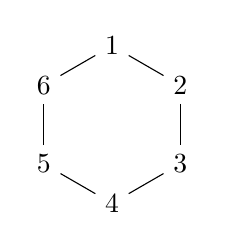
\begin{tikzpicture}
					\graph [simple] {
						subgraph C_n [n=6, clockwise];
					};
				\end{tikzpicture}
			\item Petersen graph, regular, valency 3, connected, diameter 2\\
				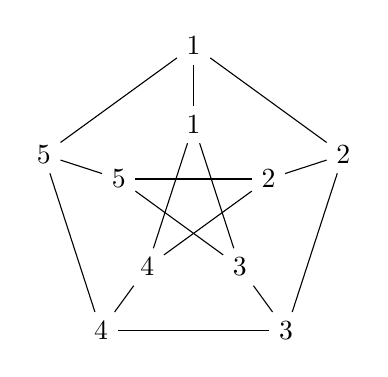
\begin{tikzpicture}
				  \graph [clockwise] {
				     subgraph C_n [n=5,name=A, radius=2cm];
				     subgraph I_n [n=5,name=B, radius=1cm];
				     \foreach \i [evaluate={\j=int(mod(\i+2,5)+1);}] in {1,...,5}{
				        A \i -- B \i;
				        B \i -- B \j;
				     }
				  };
				\end{tikzpicture}
			\item
				$diam(\Gamma) = 1 \Rightarrow \text{any 2 vertices are joined by an edge}$. Such a graph with $n$ vertices is called the \underline{complete} graph $K_n$, e.g:\\
				\begin{tikzpicture}
					\graph [simple] {
						subgraph K_n [n=3, clockwise];
					};
				\end{tikzpicture}
				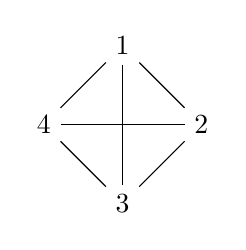
\begin{tikzpicture}
					\graph [simple] {
						subgraph K_n [n=4, clockwise];
					};
				\end{tikzpicture}

		\end{enumerate}
	\end{exmp}
	Two graphs are $(V,E)$ and $(V', E')$ are \underline{isomorphic} if there exists a bijection $V \rightarrow V'$ which sends $E \rightarrow E'$ bijectively. Eg: \\
	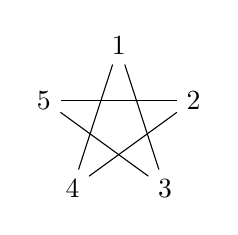
\begin{tikzpicture}
		\graph [simple] {
			subgraph K_n [n=5, clockwise];
			1 -!- 2;
			1 -!- 5;
			2 -!- 3;
			3 -!- 4;
			4 -!- 5;
		};
	\end{tikzpicture}
	$\cong$
	\begin{tikzpicture}
		\graph [simple] {
			subgraph C_n [n=5, clockwise];
		};
	\end{tikzpicture}\\

	Sometimes we write $V= V(\Gamma), E = E(\Gamma)$.

	\begin{prop}
		Suppose $\Gamma$ is a connected graph that is regular of valency $k$, diameter $d$. Then $|V(\Gamma)| \leq N(k,d) = 1 + k +  k(k-1) + k(k-1)^2 + \hdots + k(k-1)^{d-1}$
	\end{prop}
	\begin{proof}
		Let $x \in V(\Gamma)$\\
		For $i \geq 1$ let
		\[
			D_i = \{y\in V(\Gamma): d(x,y) = i\}
		\]

		Then
		\begin{align*}
			|D_1| &= k \\
			|D_2| &\leq k(k-1)\\
			|D_3| &\leq |D_2|(k-1)\leq k(k-1)^2
		\end{align*}
		and so on

		As $diam(\Gamma) = d$
		\[
			displaystyle\sum_{i=1}^{d}|D_i|V(\Gamma) = {x} \cup D_1 \cup D_2 \hdots \cup D_d
		\]
		So:
		\[
			|V(\Gamma)| \leq 1 +\sum_{i=1}^{d}|D_i| \leq 1 + \sum_{i=1}^{d} k(k-1)^{i-1}
		\]
	\end{proof}
	\begin{quest}
		When does the equality occur?
	\end{quest}
	\begin{defn}
		Call $\Gamma$ a \underline{Moore} graph if $\Gamma$ is connected, regular of valency $k$, diameter $d$ and \[|V(\Gamma)| = N(k,d)\]
	\end{defn}

	\begin{exmp}
		\begin{enumerate}
			\item $k=2, N(2,d)  =1 + 2d$\\
				\begin{figure}[H]
					\centering
					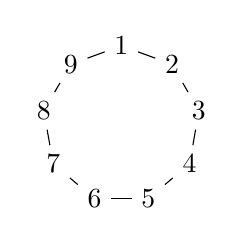
\begin{tikzpicture}
					\graph [simple] {
						subgraph C_n [n=9, clockwise];
					};
					\end{tikzpicture}
				\end{figure}
				Any \emph{$n$-gon} is a \emph{Moore Graph}

			\item $k=3, d=2, N(3,2) = 1 + 3 + 6 = 10$\\
				\begin{figure}[H]
					\centering
					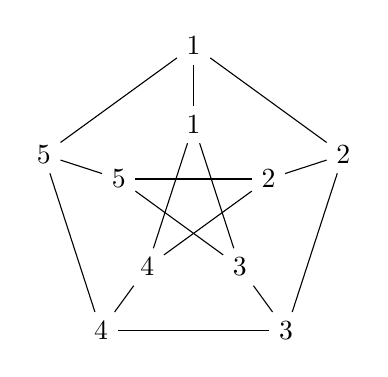
\begin{tikzpicture}
				  \graph [clockwise] {
				     subgraph C_n [n=5,name=A, radius=2cm];
				     subgraph I_n [n=5,name=B, radius=1cm];
				     \foreach \i [evaluate={\j=int(mod(\i+2,5)+1);}] in {1,...,5}{
				        A \i -- B \i;
				        B \i -- B \j;
				     }
				  };
				\end{tikzpicture}
				\end{figure}
				The Petersen graph is the only Moore graph wit these $k, d$ up to isomorphism. (excercise)
			\item $k=3, d=3$ and higher it gets much harder.
			\item $k=4, d=2$ Note that:
				\[
					N(k,2) = 1 + k + k(k-1) = k^2 + 1
				\]
				So we need a graph with 17 vertices. There is no such Moore graph with $k=4, d=2$.
				\begin{proof}
					\begin{enumerate}
						\item IN a moore graph with $diam(2)$ there are no triangles or squares
						\item Now let $k=4$. Start with an edge $0, \infty$. Let $a,b,c$ and $x,y,z$ be the other neighbours of $0$ and $\infty$.
						% TODO fix
						% \begin{figure}[H]
						% 	\centering
						% 	\begin{tikzpicture}
						%      \foreach \pos/\name in {
						%      	{(0,1)/a}, {(0,0)/b}, {(0,-1)/c},
      %                       	{(1,0)/0}, {(2,0)/infty}, {(3,-1)/z}, {(3,0)/y},{(3,1)/x}}
      %   					\node[vertex] (\name) at \pos {$\name$};
						% 	\end{tikzpicture}\\
						% \end{figure}

						As diameter is 2, $\exists$ a common neighnour of $a,x$. By (1) it's a new vertex, $call it (a,x)$.\\
						Similarly there are new vertices $(a,x), (a,y), (a,z), \hdots, (c,z)$ (9 in total). These together with $a,b,c,x,y,z,0,\infty$ are 17 vertices.

						There are 2 neighbourso f$(a,x)$ among the 9 new vertices, not $(a, \cdot)$ or $(\cdot, x)$ so possibilities are among
						\[
							(b,x), (b,z), (c,y), (c,z)
						\]

						Say %(a,x) - (b,y)

						Then $(a,x)$ not joined to $(b,z), (c,y)$ (no squares)\\
						So $(a,x)$ joined to $(b,y), (c,z)$.
						\\
						\underline{Neighbours of $(b,y)$}:\\
							$(b,y), (a,x)$ and 1 other. not $(a,\cdot), (\cdot,x), (b,\cdot), (\cdot,y)$. So the only possibility is $(c,z)$

						% fix labels

						\begin{figure}[H]
							\centering
							\begin{tikzpicture}
						  \graph [clockwise] {
						     subgraph C_n [n=3,name=A, radius=2cm];
						  };
						\end{tikzpicture}
						\end{figure}\underline{contradiction}
					\end{enumerate}
				\end{proof}
				\begin{quest}
					For which $k$ is there a Moore graph of dimension 2, valency $k$? So far we have seen examples for $k=2, k=3$, but impossible for $k=4$. We need more theory.
				\end{quest}
				\begin{proof}[Answer:]
					Only for $k=2,3,7,57$
				\end{proof}

		\end{enumerate}
	\end{exmp}

	\begin{defn}A graph $\Gamma$ is \underline{\emph{strongly regular}} with parameters $(v,k,a,b)$ if:
		\begin{enumerate}
			\item $\Gamma$ has $v$ vertices and is \underline{regular} of valency $k$.
			\item Any two joined vertices have exactly $a$ common neighbours.
				% the minimum simplex in the dual graph has a sides?
			\item any two non-joined vertices have $b$ common neighbours.
		\end{enumerate}
	\end{defn}

	\begin{prop} Suppose $\Gamma$ is strongly regular.
		\begin{enumerate}
			\item if $b > 0$ then $\Gamma$ is connected and $diam(\Gamma) = 2$
			\item if $b = 0$ then $\Gamma$ is a disjoint union of complete graphs $K_{k+1}$
		\end{enumerate}
	\end{prop}

	\begin{proof}
		\begin{enumerate}
			\item If $b>0$ then any 2 non-joined vertices can be joined by a path of length 2.
			\item Suppose $b=0$. Let vertex $x$ have neighbours $v_1,\hdots,v_k$. As $b=0$, $v_i$ is joined to $v_j,\;\forall i\neq j$. So $x,v_1,\hdots,v_k$ form a complete graph $K_{k+1}$. Any further vertex is not joined to $x$ and is not joined to any vertices $v_i$ as $b=0$.\\
			As above $y$ and its neighbours form another $K_{k+1}$
			%TODO draw it
		\end{enumerate}
	\end{proof}

	\begin{exmps}
		\begin{enumerate}
			\item Moore graphs of diameter 2 are strongly regular with parameters $(v,k, 0,1)\qquad (v=k^2+1)$ (since there are no triangles or squares). %TODO use symbols
			\item \underline{Triangular graphs $T(n)$} $(n\geq 4)$\\
			\begin{align*}
				\text{Vertices:}\; &= \binom{n}{2}\; \text{pairs from}\; \{1,\hdots, n\}\\
				\text{Edges:}\; &= \text{join}\; ij, kl\; \text{iff}\; |ij \cap kl| = 1\\
			\end{align*}
			This is a strongly regular graph with parameters

			\begin{align*}
				v &= \binom{n}{2}\\
				k &= 2n -1\\
				a &= n-2\\
				b &= 4
			\end{align*}
			% TODO get figure here
			\item \underline{Lattice graphs $L(n)$}
			\begin{align*}
				\text{Vertices:}\; &=\;\text{ordered pairs}\; (i,j),\; \text{where}\; i,j \in \{1,\hdots,n\}\\
				\text{Edges:}\; &= \text{join}\; (i,j), (k,l)\;\text{if}\; i=k\;\text{or}\; j=l\\
			\end{align*}
			Params:
			\begin{align*}
				v &= n^2\\
				k &= 2n -2\\
				a &= n-2\\
				b &= 2
			\end{align*}
			\item \underline{Payley graphs}\\
			Let $n>2$ be prime. Recall $\ZZ_p = \{0,1,\hdots, p-1\}$ with $(+,\times)$ modulo $p$ is a \underline{field}.
			\par{Define:}\\
				\[Q= \{x^2:x \in \ZZ_p^{*}\}\]
				a subgroup of $(\ZZ_p^{*}, \times)$\\
				Map $\phi: x \rightarrow x^2 \qquad (\ZZ_p^* \rightarrow Q)$ is a homomorphism with kernel:
				\[
					ker(\phi) = \{x: x^2=1\} = \{x: (x-1)(x+1) = 0\} = \pm 1
				\]
				Therefore $|Q| = |im\;\phi| = \frac{|\ZZ_p^*|}{|ker\;Q|} = \frac{p-1}{2}$
			\underline{assume $p\equiv 1 mod 4$}\\
			Then $|Q|$ is even, so (by Lagrange theorem), $Q$ has an element of order 2, whicb y above must be $-1$. Hence $-1 \in Q$.

			\begin{defn} Payley graph $P(p)$, $(p\;\text{prime}\;\equiv 1 mod 4)$\\
			\begin{align*}
				\text{Vertices:}\; &=\;\text{elements of $\ZZ_p$}\; (i,j),\; \text{where}\; i,j \in \{1,\hdots,n\}\\
				\text{Edges:}\; &= \text{join}\; (x,y)\; \text{iff $(x,y) \in Q$}\\
			\end{align*}
			\begin{figure}[H]
				\centering
				\begin{tikzpicture}
				\graph [simple] {
					subgraph C_n [n=5, clockwise];
				};
				\end{tikzpicture}
			\end{figure} is the smallest Payley graph
			\end{defn}
		\end{enumerate}
		\begin{prop} $P(p)$ is strongly regular, params:
		\[
		v =p, \quad k = \frac{p-2}{2}, \quad a=\frac{p-5}{4},\quad b=\frac{p-1}{4}
		\]
		\end{prop}
		\begin{proof} See sheet 4
		\end{proof}
	\end{exmps}
	\subsection{Theory}
		\begin{prop} If $\Gamma$ is strongly regular, params $(v,k,a,b)$ then $\Gamma^C$ is also strongly regular, params $(v,v-k-1, v-2l+b-2, v-2k+1)$.[$\Gamma^C$, the \underline{complement} of $\Gamma$ is the graph with the same vertex set and all edges (non-edges) replaced with non-edges (edges), Eg. $P(5)$ is the complement of $K_5 - P(5)$].
		\end{prop}

		\begin{proof} $\Gamma^C$ is regular of valency $v-k-1$ (as we are connecting each vertex to $v-1-k$ vertices that were previously disconnected).\\

		In $\Gamma^C$, $b$ becomes:
		\[
			v - 2(k-a-1) -a- 2 = v-2k + a
		\]
		Since we are removing $2(k-a-1)$ common neighbours and we are disconnecting an extra pair $a-2$
		\\
		Param $a$ is $v-2(k-b)-b-2 = v -2k + b -2$
		\end{proof}
		\begin{prop}{Balloon equation}
		If $\Gamma$ is strongly regular graph with params $(v, k, a, b)$, then:
		\[k(k-a-1) = b(v-k-1)\]
		\end{prop}
		\begin{proof}
			Let $x \in V(\Gamma)$, let $A$ be the set of  $k$ neighbours of $x$, and $B$ be the remaining vertices.
			\begin{figure} %TODO fix figure
				\begin{tikzpicture}
					\begin{pgfonlayer}{nodelayer}
						\node [style=none] (0) at (-3.75, 0) {$x$};
						\node [style=none] (1) at (-2, 1) {};
						\node [style=none] (2) at (-2, 0) {};
						\node [style=none] (3) at (-2, -1) {};
						\node [style=none] (4) at (2, 1.5) {};
						\node [style=none] (5) at (2, 0.5) {};
						\node [style=none] (6) at (2, -0.5) {};
						\node [style=none] (7) at (2, -1.5) {$B$};
						\node [style=none] (8) at (-2, -2) {$A$};
					\end{pgfonlayer}
					\begin{pgfonlayer}{edgelayer}
						\draw [style=dashed] (0.center) to (1.center);
						\draw [style=dashed] (0.center) to (2.center);
						\draw [style=dashed] (0.center) to (3.center);
						\draw [style=dashed] (1.center) to (4.center);
						\draw [style=dashed] (1.center) to (5.center);
						\draw [style=dashed] (3.center) to (6.center);
					\end{pgfonlayer}
				\end{tikzpicture}
			\end{figure}
			So $|B| = v - k -1$.\\
			Count the number of edges between $A$ and $B$. Each vertex in $A$ is joined to $k-a-1$ vertices in $B$, so:
			\begin{align*}
				|N| &= |A| \times (k-a-1)\\
					&= k(k-a-1)
			\end{align*}
			Each vertex in $B$ is joined to $b$ vertices in $A$. So:
			\[|N| = |B| \times b = (v-k-1)b\].
			Hence $k(k-a-1) = b(v-k-1)$
		\end{proof}
		\begin{rem}
		``Balloon picture'' of $\Gamma$
		%insert pic
		e.g. Moore graphs of diameter 2 are strongly regular with parameters $(v, k, 0, 1)$. Picture %picture her
		So the ``baloon equation'' is $k(k-1) = v-k-1$. So $v = k^2 +1$
		\end{rem}
	\subsection{Adjacency matrices}
		Let $\Gamma$ be a graph with vertex set $\{e_1,\hdots, e_r\}$. Define a $r \times r$ matrix $A = (a_{ij})$ by:
		\[
			a_{ij} = \begin{cases}
						1 &\quad \text{if $e_i$ joined to $ej$}\\
						0 &\quad \text{otherwise}
					 \end{cases}
		\]

		\begin{exmp}
			\begin{figure}[H]
				\centering
				\begin{tikzpicture}
				\graph [simple] {
					subgraph C_n [n=5, clockwise];
				};
				\end{tikzpicture}
			\end{figure}
			\[
				A = \begin{pmatrix}
					0 & 1 & 0 & 0 & 1\\
					1 & 0 & 1 & 0 & 0\\
					0 & 1 & 0 & 1 & 0\\
					0 & 0 & 1 & 0 & 1\\
					1 & 0 & 0 & 1 & 0
					\end{pmatrix}
			\]
		\end{exmp}

		\par{Basic properties of $A$:}\hfill \\
			\begin{enumerate}
				\item $A$ is symmetric with all entries 0 or 1
				\item $A$ has zeroes on the diagonal
			\end{enumerate}

		\begin{defn}
			$A$ is the \underline{adjacecny matrix of} $\Gamma$
		\end{defn}

		For strongly regular graph, $A$ has nice properties.

		\begin{prop}
			Let $\Gamma$ be strongly regular, params $(v, ka, a, b)$ with the adjacency matrix $A$. Let $J$ be the $v \times v$ matrix with all entries 1.
			\begin{enumerate}
				\item $AJ = kJ$
				\item $A^2 = (a-b)A + (k-b)I + bJ$
			\end{enumerate}
		\end{prop}

		\begin{proof}
			\begin{enumerate}
				\item As $\Gamma$ is regular of valency $k$, each row of $A$ has $k$ 1s so $AJ = kJ$
				\item Since $A$ is symmetric, $A^2 = AA^T$ So:
				\begin{align*}
				  ij\text{th entry of $A^2$}\quad
				  	&= ij\text{th entry of $AA^T$}\\
				  	&= (\text{row $i$ of $A$})(\text{col $j$ of $A^T$})\\
				  	&= (\text{row $i$ of $A$})(\text{row $j$ of $A$})\\
				  	&= \text{no. of common neighbours of $e_i$ and $e_j$}\\
				  	&= \begin{cases}
				  			k \quad \text{if $i = j$}\\
				  			a \quad \text{if $i \neq j$ and $e_i$ and $e_j$ are joined in $\Gamma$}\\
				  			b \quad \text{if $i\neq j$ and $e_i$ and $e_j$ are not joined in $\Gamma$}
				  	   \end{cases}
				\end{align*}
				So $A^2$ has $k$s on the diagonal, $a's$ where $A$ has a one (i.e. where $A$ describes edges that are joined), $b's$ elsewhere.\\
				Therefore:
				\begin{align*}
					A^2 &= kI = aA + b(J-I-A)\\
						&= (a-b)A + (k-b)I + bJ
				\end{align*}
			\end{enumerate}
		\end{proof}

		\paragraph{Eigenvalues} Let $v$ is the number of vertices. Adjacency matrix of a graph $\Gamma$ is real and symmetric, so it has real eigenvalues and is diagonalizable, i.e.:
		\[
			\exists P \quad\text{s.t.}\quad 
			P^{-1}AP = \begin{pmatrix}
						\lambda_1 & & 0\\
						& \ddots & \\
						0 & & \lambda_v
						\end{pmatrix}
		\]
		The \underline{multiplicity} of an eigenvalue $\lambda_i$  is the number of times it appears on the diagonal.



		\begin{thm}[2.7]
			Let $\Gamma$ be a strongly regular graph with $(v, k, a, b)\quad b >0,\quad v> 2k$.
			\begin{enumerate}
				\item $A$ has 3 eigenvalues $k, r_1, r_2:\quad r_1, r_2$ are roots of:
					\[x^2 - (a-b) x - (k-b) = 0\]
				\item $r_1, r_2$ have multiplicities $m_1, m_2$, where:
					\begin{align*}
						m_1 + m_2 &= v-1\\
						m_1 r_1 + m_2 r_2 = 0k\\
					\end{align*}
				\item $r_1, r_2 \in \ZZ$, unless parameters $(4b +1,2b, b-1, b)$
			\end{enumerate}
		\end{thm}
		\begin{rem}Concerning the 2nd assumption: $v > 2k$\\
			If $2k \geq v$ then $\Gamma^C$ is strongly regular (proven last time) with params $(v, v-k-1, \hdots)$ adn $v \leq 2k \Rightarrow v > 2(v-k-1)$ where $v -k-1$ is the valency of $\Gamma^C$
			So Theorem 2.7 applies to $\Gamma^C$ provided $\Gamma^C$ is connected (i.e. $b > 0$). If $\Gamma^C$ is not connected we know from (2.3) that $\Gamma^C$ is a disjoin union of complete graphs, so we know what $\Gamma$ is.
		\end{rem}

		\paragraph{\emph{Proof later}}

		\subsubsection*{Applications}
			\paragraph{Moore graphs}: Recall Moore graph of diameter 2 is strongly regular, parameters $(v, k, 0, 1), v=k^2 +1$
				\begin{thm}[2.8]
					If $\exists$ a Moore graph of valency $k$ diameter 2, then:
					\[
						k = 2,3,5,6\; \text{or}\; 57
					\]
				\end{thm}
				\begin{proof}
					Let $\Gamma$ be sucha Moore graph, so $\Gamma$ is strongly regular, params $(k^2 +1, k, 0, 1)$. Note $b = 1 > 0$ and $k^2 + 1 > 2k$  ( as$k > 1$). So Theorem 2.7 applies. Let $A$ be the adjacency matrix of $\Gamma$. By 2.7 $A$ has 3 eigven values $k, r_1, r_2$ where $r_1, r_2$ are the roots of:
					\[x^2 + x - (k-1) = 0\]
					So:\[r_1, r_2, = \frac{1}{2}\left( -1 \pm \sqrt{4k-3}\right)\]
					\\
					By 2.7 (2) the results $m_1, m_2$ of $r_1, r_2$ satisfy:
					\begin{align*}
						m_1 + m_2 &= k^2\\
						m_1 r_1 + m_2 r_2 &= -k
					\end{align*}

					From the second equation we get:
					\[
						\frac{1}{2}\left(-m_1 -m_2\right) + \frac{1}{2}\sqrt{4k-3}\left( m_1 - m_2\right) = -k
					\]
					So:
					\[
						\sqrt{4k - 3}\left(m_1 - m_2\right) = k^2 - 2k
					\]
					But we also know that the square root term is an integer, which gives us a lot of information about $k$

					By 2.7(3) $r_1, r_2 \in \ZZ$ unless the parameters are $(5, 2, 0, 1)$, in which case $\Gamma$ is $C_5$ (a pentagon). Therefore $r_1, r_2 \in \ZZ$. This implies $\sqrt{4k-3} \in \ZZ$ Write:
					\[
						n = \sqrt{4k-3}
					\]
					Then $n^2 = 4k - 3$, so $k = \frac{n^2 + 3}{4}$. Then use it in the previous equations:

					\begin{align*}
						n(m_1 - m_2) &= k(k-2)\\
									 &= \frac{n^2+3}{4} \times \frac{n^2-5}{4}
					\end{align*}

					Conclude that $m_1 - m_2 = \frac{(n^2+3)}{(n^2-5)}{16n}$.

					Key point: this is an integer. So $n$ divides $(n^2+3)(n^2 - 5)$.
					Now:

					\begin{align*}
						hcf(n, n^2+3) &| 5\\
						hcf(n, n^2-5) &|5\\
					\end{align*}
					Therefore $n$ divides 15. Possibilities:
					\begin{description}
						\item{$n = 1$} then $1 = \sqrt{4k-3} \Rightarrow k = 1$ \underline{contradiction}
						\item{$n = 3$} then $4k-3 = 9 \Rightarrow k = 3$
						\item{$n = 5$} then $4k-3 = 25 \Rightarrow k = 7$
						\item{$n = 15$} then $4k-3 = 225 \Rightarrow k = 57$
					\end{description}
				\end{proof}
			\paragraph{Frendship theorem}
				\begin{thm}
				Suppose $\Gamma$ is a graph in which any 2 vertices have exactly 1 common neighbour. Then $\exists$ a vertex that is joined to all of the other verices.
				\end{thm}
				\begin{proof}
					Assume false, i.e. there is \underline{no vertex} that is joined to all the others. Aim for contradiction.
					\begin{clm}$\Gamma$ is a regular graph
					\end{clm}
					\begin{proof}
						First we show, if $P, Q$ are non-joined vertices, then $v(P) = v(Q)$ (where $v(P) = $ no. of the neighbours of $P$).


						To see this, let $R$ be the common neighbour of $P$ and $Q$. Let $S$  be the common neighbour of $P, R$ and $T$ a common neighbour of $Q,R$. Note that $S \neq T$ (otherwise $P,Q$ would have 2 common nieghbours). Let the remaining neighbours of $P$ be $u_1, u_2, \hdots, u_r$. Consider the common neighbour of $u_1$ and $Q$. It is not $T$ (otherwise $P,T$ have 2 common neighbours) and it is not $R$, (otherwise $P,R$ have 2 common nieghbours). So it is a new vertex $v_1$. Now consider the common neighbour of $u_2, Q$. It's not $v_1$ (otherwise $u_1, u_2$ have 2 common neighbours). So it is a new vertex $v_2$. Carrying on for each $u_i$, its common neighbour with $Q$ is a new vertex $v_i$
						\begin{figure}
							\centering
							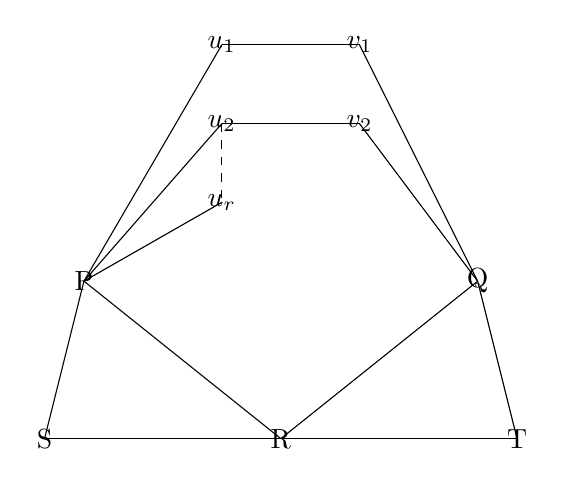
\begin{tikzpicture}
								\begin{pgfonlayer}{nodelayer}
									\node [style=dashed] (0) at (-2.5, 0) {P};
									\node [style=dashed] (1) at (2.5, 0) {Q};
									\node [style=dashed] (2) at (0, -2) {R};
									\node [style=dashed] (3) at (-3, -2) {S};
									\node [style=dashed] (4) at (3, -2) {T};
									\node [style=dashed] (5) at (-0.75, 3) {$u_1$};
									\node [style=dashed] (6) at (-0.75, 2) {$u_2$};
									\node [style=dashed] (7) at (-0.75, 1) {$u_r$};
									\node [style=dashed] (8) at (1, 3) {$v_1$};
									\node [style=dashed] (9) at (1, 2) {$v_2$};
									\node [style=dashed] (10) at (1, 2) {};
								\end{pgfonlayer}
								\begin{pgfonlayer}{edgelayer}
									\draw (0.center) to (2.center);
									\draw (2.center) to (1.center);
									\draw (0.center) to (3.center);
									\draw (3.center) to (2.center);
									\draw (2.center) to (4.center);
									\draw (4.center) to (1.center);
									\draw (0.center) to (5.center);
									\draw (0.center) to (6.center);
									\draw (0.center) to (7.center);
									\draw (5.center) to (8.center);
									\draw (8.center) to (1.center);
									\draw [style=dashed] (6.center) to (7.center);
									\draw (6.center) to (9.center);
									\draw (9.center) to (1.center);
								\end{pgfonlayer}
							\end{tikzpicture}
						\end{figure}
						Hence:
						\[
							v(P) = r+2 \leq v(Q)
						\]
						Similarly $v(Q) \leq v(P)$, hence $v(P) = v(Q)$ proving the claim.
					
					First note that non-joined $P,Q$ exist (by the assumption that $\exists$ a vertex joined to all others). So $v(P) = v(Q)$. Let $R$ be a common neighbour of $P,Q$. If $S$ is a futher vertex it is not joined to both $P, Q$ by the previous claim. Moreover
					\[ v(S) = v(P) = v(Q)\]
					Finally by assumption $\exists$ vertex $S$ not joined to $R$, so $v(R) = v(S)$. Therefore $\Gamma$ is regular.
					\end{proof}
					\begin{clm}{last part} $\Gamma$ is strongly regular with params $(v, k, 1, 1)$
					\end{clm}
					\begin{clm} There is no such strongly regular graph
					\end{clm}

					\begin{proof}
					% balloon pic (1) -1- (k) -k-2 - 1 (v-k-1)
					% (k) - 1 - (k)
					So:
					\[k(k-2) = v-k-1\]
					Hence:
					\[v=k^2-k+1\]
					Now apply Theorem 2.7. Note:
						\begin{itemize}
							\item $b = 1 > 0$
							\item $v = k^2-k +1 > 2k \Leftrightarrow k \geq 3$
						\end{itemize}
					If $k =2$ then $v = 3$ and $\Gamma$ is $C_3$. \underline{contradiction}\\
					Hence $v > 2k$, so Theorem 2.7 applies to $\Gamma$
					Let $A$ be the adjacency matrix of $\Gamma$.\\
					By 2.7(1), $A$ has 3 eigenvalues $k, r_1, r_2$, wher $r_1, r_2$ are the roots of:
					\[ x^2 - k(-1) = 0\]
					So $r_1 = \sqrt(k-1),\quad r_2 = -\sqrt(k-1)$
					By 2.7 (2), multiplicities $m_1, m_2$ of $r_1, r_2$ satisfy:
					\begin{enumerate}
						\item $m_1 + m_2 = k^2 -k$
						\item $r_1 m_1 + r_2 m_2 = -k$
					\end{enumerate}
					From (2):
					\[ \sqrt{k-1}(m_1 - m_2) = -k\]
					Hence:
					\[(k-1)(m_1-m_2)^2 = k^2\]
					Since $m_1 - m_2 \in \ZZ$, this means $k-1$ divides $k^2$.
					But $hcf(k-1, k) = 1$, so there is no such strongly regular graph unless $k = 2$.
					\end{proof}
				\end{proof}
			\paragraph{Strongly regular graphs with small $v$}
				\begin{quest} What are the possible parameters of strongly regualr graphs with $v = 15$
				\end{quest}
				\begin{exmps}
					\begin{enumerate}
						\item Triangular graph $T(6)$: vertices are pairs from $\{1,\hdots, 6\}$, join $ij$ with $kl$ if $|ij \cap kl| = 1$. Params of $T(6)$ are $(15, 8, 4, 4)$
						\item $T(6)^C$: params $(16, 6, 1, 3)$
						\item Examples with $b= 0$: $(K_3)^5$ and $(K_5)^3$. Parameters are $(15, 2, 1, 0)$, $15, 4, 3, 0$ respectively.\\
						Complements of these are also strongly regular with $v = 15$, paramters are: $(15, 12, 9 ,12)$, $(15,10, 5, 10)$ respectively.
					\end{enumerate}
				\end{exmps}
				\begin{prop}
					If $\Gamma$ is strongly regular with $v = 15$ then $\Gamma$ is isomorphic one of the graphs listed above. I.e. the parameters of $\Gamma$ are those of $T(6), (K_5)^3, (K_3)^5$ or of the complements of those.
				\end{prop}
				\begin{proof}
					Let $\Gamma$ have parameters$(15, k, a, b)$ If $15 \leq 2k$, replace $\Gamma$ by complement $\Gamma^C$ so can assume:
					\[ 15 > 2k\]
					If $b=0$ then $\Gamma$ is $(K_5)^3$ or $(K_3)^5$ by (2.2)
					So assume now that $b>0$. Hence Theorem 2.7 applies to $\Gamma$\\
					Consider each possible $k$, with $2 \leq k \leq 7$
					\begin{description}
						\item[$k=2$] $\Gamma$ is a 15-gon, which not strongly regular \underline{contradiction}
						\item[$k=3$] Balloon:
							%(1) - (3) - (11) 
							By balloon equation
							\begin{align*}
								3(2-a) = 11b &\Rightarrow 11 | 3(2-a) \\
									&\Rightarrow 11 | 2-a \\
									&\Rightarrow a = 2
							\end{align*}
							\underline{contradiction}
						\item[$k=4$] Balloon:
							%(1) - (4) - (10) 
							By balloon equation
							\begin{align*}
								4(3-a) = 10b &\Rightarrow 10 | 4(3-a) \\
									&\Rightarrow 5 | 3-a \\
									&\Rightarrow a = 3
							\end{align*}
							\underline{contradiction}
						\item[$k=3$] Balloon:
							%(1) - (5) - (9) 
							By balloon equation
							\begin{align*}
								5(4-a) = 9b &\Rightarrow 9 | 4-a \\
									&\Rightarrow a = 4, b =0
							\end{align*}
							\underline{contradiction}
						\item[$k=6$]
							\[6(5-a) = 8b \Rightarrow a=1, b = 3 \]
							These are the parameters $(15, 6, 1, 3)$ so, $\Gamma \cong T(6)^C$
						\item[$k=7$]
							%(1) - (7) - (7) 
							Here $7(6-a) = 7b \Rightarrow b = 6 - a$\\
							Apply Theorem 2.7:
							The eigenvalues are $7, r_1, r_2$, roots of:
							\begin{align*}
								x^2 - (a - b) x - (k -6 ) &= 0\\
								x^2 - (2a - 6) x - (a + 1) &= 0\\ 
							\end{align*}
							So $r_1,r_2 =  (a-3)\pm \sqrt(a^2 - 5a + 10)$. Use part 3 of Theorem 2.7. These are integers, since $15 \neq 4b + 1$.
							$r_1, r_2 \in \ZZ$ hence: $a^2 -5a + 10$ is a square. We know that $0 \leq a \leq 5$. Possible such $a$ are: $2, 3$. 
							\begin{description}
								\item[$a= 2$] Then $r_1 = 1, r_2 = -3$, so 2.7(2) gives $m_1 + m_2 = 14$ and $m_1 - 3m_2 = -7$
								So $4m_2 = 21$, But $m_2 \in \ZZ$\underline{contradiction}
								\item[$a = 3$] Then $r_1 = 2, r_2 = -2$. And $m_1 + m_2 = 14$, $2_m1 - 2m_2 = -7$ \underline{contradiction}
							\end{description}
							So $k = 7$ does not occur.
					\end{description}
				\end{proof}
				\paragraph{Proof of Theorem 2.7}
				We are going to need:
				\begin{lem} Let $A$ be a $v \times v$ real matrix $(a_{ij})$. and let $\lambda_1, \hdots, \lambda_v$ be the eigenvalues of $A$. Then $Tr(A) = \sum_{i=1}^{v} \lambda_i$
				\end{lem}
				\begin{proof}
					By definition, $\lambda_i$ are the roots of the characteristic polynomial of $A$:
					\begin{align*}
						|xI - A| &= det\left(\begin{bmatrix}
									x - a_{11}& -a_{12} &\hdots& x- a_{1v}\\
									-a_{21}& x-a_{22} &\hdots& x- a_{2v}\\
									& &\vdots &\\
									-a_{v1} & \hdots & \hdots & x-a_{vv}\\
								   \end{bmatrix}\right)\\
								 &= x^v + x^{v-1}(-a{11} - \hdots - a_{vv})\\
								 &= x^v - Tr(A) x^{v-1} + \hdots
					\end{align*}
					Therefore the sum of the roots is $Tr(A)$
				\end{proof}

		% missing monday 2.04.2014

		Let's clear up a point:

		The complete graph $K_n, K_n^C$ do not count as strongly regular graphs. 
	\subsection{Two-weight codes and strongly regular graphs}
		\begin{defn}
			A linear code $C \subseteq \ZZb^n$ is a \underline{two-weight} code if $\exists$ positive integers $w_1, w_2, w_1 \neq w_2$ such that every non zero codeword in $C$ has a weight $w_1$ or $w_2$ and both weights occur.
		\end{defn}

		\begin{exmps}\hfill
			\begin{enumerate}
				\item Extended $Ham(3) \subseteq \ZZb^8$ weights 4, 8
				\item $C = \left\{v \in \ZZb^5 : wt(v)\; \text{is even} \right\}$ weights 2,4
				\item $C = \left\{ x \in G_{24} : x_{16} = \hdots = x_{24} = 0\right\}$ weights 8, 12
			\end{enumerate}
		\end{exmps}

		\paragraph*{Recall:} a \underline{generator matrix} for a linear code is a matrix whose rows form a basis for the code.

		\begin{defn}
			A linear code is \emph{projective} if it has a generator matrix with all columns distinct and nonzero
		\end{defn}

		\begin{exmp} $H'$ is a projective generator matrix:
		\[
			\begin{matrix}
				1 & 1 & 1 & 1 & 1 & 1 & 1 & 1\\
				0 & 1 & 1 & 1 & 0 & 0 & 0 & 1\\
				0 & 1 & 0 & 0 & 1 & 1 & 0 & 0\\
				0 & 0 & 1 & 0 & 1 & 0 & 1 & 1
			\end{matrix}
		\]
		\end{exmp}

		\begin{thm}[2.12]
			Let $C \subseteq \ZZb^n$ be a linear code and assume:
			\begin{itemize}
				\item $C$ is projective
				\item $C$ is a two-weight, with weights $w_1 < w_2$
			\end{itemize}

			Define a graph $\Gamma$ as follows:

			\begin{itemize}
				\item vertices of $\Gamma$ : codewords in $C$
				\item join vertices $a, b$ : if and only if $d(a, b) = wt(a + b) = min(w_1, w_2)$
			\end{itemize}
			Then $\Gamma$ is a strongly regular graph.
		\end{thm}

		\begin{exmp} $C = H'$ (extended Hamming(3) code), $w_1 = 4, w_2 = 8$.\\
		What is $\Gamma$?\\
		Well in $\Gamma^C$ we join codewords $a, b$ if and only if $d(a,b) = 8$, i.e. $a = b + 1^8$. So $a$ is joined to only one other vector. So valency of $\Gamma^C$ is 1 and it is $K_2^8$
		\end{exmp}

		\begin{proof}\hfill\\
			Let $k = dim(C)$ and let $b_1, b_2$ be the number of codewords in $C$ of weight $w_1, w_2$ respectively.\\
			Note $b_1 + b_2 = |C| - 1 = 2^k - 1$ (ommitting the zero vector)\\
			For $i = 1, 2$ let:
			\[
				A_i = b_i \times n\ \text{matrix whose rows are the codewords of wt $w_i$}
			\]
			Define:
			\[
				A = \begin{pmatrix}
					\begin{array}{cc}
					A_1\\ \hline
					A_2
					\end{array}
					\end{pmatrix} \quad (b_1 + b_2) \times n
			\]
			\begin{clm}
				Each column of $A$ hs weight $2^{k-1}$
			\end{clm}
			
			\begin{proof}
				Define $\phi_i : C \rightarrow \ZZb$ by:
				\[
					\phi_i(x_1,\hdots,x_n) = x_i				
				\]
				$\forall i$ the $i^{th}$ column of $A$ is non zero (as $C$ is projective), so $\phi_i$ is surjective. Therefore $ker\phi_i$ has dimension $k-1$\\
				Hence the $i^{th}$ column of $A$ has $2^{k-1} - 1$ zeros and the rest of the entries are $2^{k-1}$ ones.\\
			\end{proof}
			
			Now we have equations:
			\begin{align*}
				b_1 + b_2 &= 2^k-1\\
				b_1w_1 + b_2 w_2 &= n2^{k-1}
			\end{align*}

			Hence we can work out $b_1, b_2$.
			\paragraph*{Next step}
				Consider column $j$ of $A$. Let $r_1$ be the number of 0's in col $j$ of $A_1$ and $r_2$ the number if 0's in col $j$ of $A_2$. Codewords in $C$ with 0 in $j^{th}$ position form a subcode of $C$ which is two-weight, with weights $w_1 -1, w_2 -1$. Its generator matrix has no zero column. (we are dropping the $j^{th}$ column however) \\
				Otherwise $A$ would have another column identical to $j$, but $C$ is assumed to be projective, so it can't have two identical columns.

				Hence we can work out $r_1, r_2$ as for $b_1, b_2$. $r_1, r_2$ are independent of the choice of column $j$. So every column of $A_i$ has $r_i$ 0's. 

			\paragraph*{Bring back the graph}
				Let us label the rows of $A_1$ as $a_1, \hdots, a_{b_1}$. (recall $b_1 + b_2 = k$ and $b_1$ is number of rows in $A_1$) We can calculate:
				\[
					\sum_{i=1}^{b_1} d(a_i, a_1) = D
				\]

				Let:
				\begin{align*}
					s_1 &=\ \text{number of $a_i$'s such that $d(a_1, a_i) = w_1$}\\
					s_2 &=\ \text{number of $a_i$'s such that $d(a_1, a_i) = w_2$}\\
				\end{align*}
				Then:
				\begin{align*}
					s_1 + s_2 &= b_1 -1 \\
					s_1 w_1 + s_2 w_2 &= D
				\end{align*}

				So can calculate $s_1, s_2$.
				Now in the graph $\Gamma:$
					\begin{figure}[H]
						\centering
						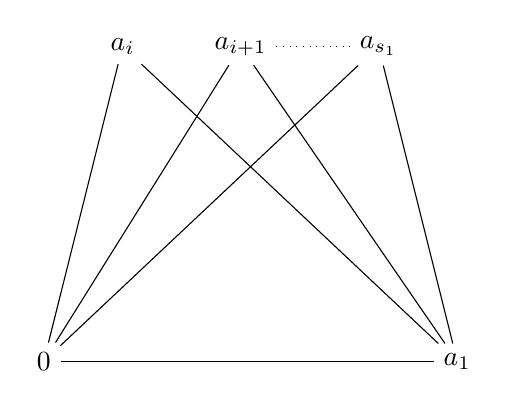
\begin{tikzpicture}
							\begin{pgfonlayer}{nodelayer}
								\node (0) at (-2.75, -1.25) {0};
								\node (1) at (2.5, -1.25) {$a_1$};
								\node (2) at (-1.75, 2.75) {$a_{i}$};
								\node (3) at (-0.25, 2.75) {$a_{i+1}$};
								\node (4) at (1.5, 2.75) {$a_{s_1}$};
							\end{pgfonlayer}
							\begin{pgfonlayer}{edgelayer}
								\draw  (0) to (1);
								\draw  (0) to (2);
								\draw  (0) to (3);
								\draw  (3) to (1);
								\draw [style=dotted] (3) to (4);
								\draw  (4) to (1);
								\draw  (4) to (0);
								\draw  (2) to (1);
							\end{pgfonlayer}
						\end{tikzpicture}
					\end{figure}
				SO for any edge such that the corresponding codeword $c$ has weight $w_1 = wt(c)$

					\begin{figure}[H]
						\centering
						\begin{tikzpicture}
							\begin{pgfonlayer}{nodelayer}
								\node (0) at (-2.75, -1.25) {0};
								\node (1) at (2.5, -1.25) {$c$};
							\end{pgfonlayer}
							\begin{pgfonlayer}{edgelayer}
								\draw (0) to (1);
							\end{pgfonlayer}
						\end{tikzpicture}
					\end{figure}
				The vertices $0, c$ have $s_1$ common neighbours.

				For a general edge $x \longleftrightarrow y, wt(x+y) = w_1$ there is a bijective correspondence between common neighbours of $x,y$ and those of $0, x+y$

				So any joined pair $x, y$ have $s_1$ common neighbours.
				Similarly working with $A_2$ see that any non-joined pair has constant number of common neighbours, Finally note $\Gamma$ is regular of valency $b_1$. Hence $\Gamma$ is strongly regular.
		\end{proof}


\section{t-designs}
% $missing 8.9.15
	\subsection{Symmetric 2-designs}
		\begin{defn}
			A 2-design is symmetric if it has $b = v$. Equivalently $k = r$
		\end{defn}

		\begin{exmp}
			$X = \ZZb^3 \setminus 0, |X| = 7$
			Block one sets $\{x,y, x+y\}$
			This is a 2-design params $(7,3,1)$
			For this design
			\[
				\lambda(v-1) = r(k-1) \Rightarrow b = r \Rightarrow r = 3
			\]
			So $b = \frac{vr}{k} = 7$. So this is symmetric

			This is called a \underline{Fano plane}.

			% pic of fano plane

			This is the smallest \underline{projective plane} symmetric 2-design with $\lambda = 1$
		\end{exmp}

		\begin{thm}
			Suppose there exists a symmetric 2-design with params $(v, k, \lambda)$, and $v$ is even. Then $k-\lambda$ is a square.
		\end{thm}

		\begin{exmp}
			Is there a 2-design with params $(22, 7, 2)$?
		\end{exmp}
			\paragraph*{Answer:} Well:
				\[
					\lambda(v-1) = r(k-1) \implies 2 \times 21 = r \times 6 \implies r = 7 = k
				\]

				But $v = 22$ is even and and $k-\lambda = 7 - 2 = 5$ is not a square. So no such design exists

		\begin{proof}
			As $b = v$, the incidence matrix for $A$ is square $v \times v$. So $det(A)$ exists and moreover, since $A$ is square, $det(A) \in \ZZ$. \\

			Now $det(A^T) = det(A)$, so $det(AA^T) = det(A)^2$.
			By Proposition (3.5)
			\[
				det(A)^2 = (r - \lambda)^2(\lambda(v-1) + r)
			\]

			Now noting that $r = k$
			\[
				\lambda(v-1) = r(k-1) = k(k-1)
			\]
			So

			\[
				\lambda(v-1) + r = k(k-1) + k = k^2
			\]

			Hence 
			\[
				det(A)^2 = (k - \lambda)^{v-1}k^2
			\]
			Both sides are squares in $\ZZ$, hence $(k-\lambda)^{v-1}$ is a square. As $v$ is even, $v-1$ is odd, so $k-\lambda$ is a square.
		\end{proof}
					
		\begin{rem}
			If $v$ is odd, the \underline{Bruch-Ryser-Charla} theorem says: if a symmetric 2-design exists with parameters $(v, k, \lambda)$ then the equation:
			\[
				z^2 = (k-\lambda)x^2 + (-1)^{\frac{v-1}{2}}\lambda y^2
			\]
			has a solution with $x,y,z \in \ZZ$ (not all $x,y,z = 0$)
		\end{rem}					
		
		\begin{thm}(3.10)
			If $\mathcal{B}$ is a symmetric 2-design with parameters $(v,k, \lambda)$, then any 2 blocks of $\mathcal{B}$ intersect in exactly $\lambda$ points.
		\end{thm}

		\begin{proof}
			Let $A$ be the $v \times v$ incidence matrix. Consider $A^T A$:
			\begin{align*}
				\text{$ij$-entry} &= (\text{row $i$ of $A^T$}) \cdot (\text{col $j$ of $A$})\\
								  &= (\text{col $i$ of $A$}) \cdot (\text{col $j$ of $A$})\\
								  &= |B_i \cap B_j|
			\end{align*}

			Where $\mathcal{B} = \{B_1, \hdots, B_v\}$
			ON the other hand by 3.5
			\[
				AA^T = \begin{pmatrix}
				 		r & \lambda & \hdots & \lambda \\
				 		\lambda & r & \hdots & \lambda \\
				 		\vdots & & \ddots & \\
				 		\lambda & & & r
						\end{pmatrix} = \lambda J + (r-\lambda) I
			\]

			So we are done if we prove $A^T A = A A^T$.
			Now $AJ = kJ = JA$ and $AI = IA$ hence A commuts with $A A^T = \lambda J + (r - \lambda) I$. So

			\[AAA^T = A A^T A\]
			We know that $det(AA^T) = det(A)^2$ = $(k-\lambda)^{v-1}k^2 \neq 0$. So $det(A) \neq 0$. So $A$ is invertible and we can cancel out $A$ on the left in the equality above, so $AA ^T = A^T A$. 
		\end{proof}

		\paragraph*{Projective planes}
			A symmetric 2-design with $\lambda = 1$ is called a projective plane. By 3.10 any two blocks will meet in 1 point. 

			\begin{defn}(Equivalent definition of a projective plane)\hfill\\
				A set of points and lines (lines are the blocks, or subsets of points) satisfying 3 axioms:
				\begin{enumerate}
					\item Any 2 points lie on a unique line
					\item Any 2 lines meet in a unique point
					\item There exists a collection of 4 points such that no 3 are on the same line
				\end{enumerate}
			\end{defn}

			\begin{rem}
				Follows from the axioms that all lines have the same number of points. So a projective plane is indeed a 2-design with $\lambda = 1$ - can show that it is also symmetric.
			\end{rem}

			\begin{rem}
				There is a converse to theorem 3.9 - namely, if there exists a 2-design with $(v, k, \lambda)$ in which any 2 blocks intersect in $\lambda $ points, then it is automatically symmetric.
			\end{rem}

	\subsection{Examples of symmetric 2-designs}\hfill\\		
		\subsection*{Difference sets}
			\begin{exmp}
				Let $X = \ZZ_7 = \{0, 1, \hfill, 6\}$ and let $B_0 = {0, 1, 3} \subset X$\\
				Define 7 subsets of $X$:

				\[
					B_0 + i = \{b+i\ :\ b \in B_0\} \quad (0 \leq i \leq 6)
				\]

				These subsets are:
				\[
					\{0, 1, 3\}, \quad \{1, 2, 4\}, \quad \{2, 3, 5\},\quad \hdots \quad \{6,0,2\}
				\]
			\end{exmp}
			\begin{clm} The subsets $B_0 + i,\ (0 \leq i \leq 6)$ are the blocks of a symmetric 2-design, params $(7,3,1)$
			\end{clm}

			\begin{proof}
				Consider the differences $b_1 - b_2$ for $b_1, b_2 \in B_0,\ b_1 \neq b_2$. Easy inspection shows that each non zero element of $\ZZ_7$ occurs exactly once as a difference. The claim holds by proposition below
			\end{proof}

			\begin{defn}
				Let $\lambda$ and $v$ be positivive integers and let $B_0 \subseteq \ZZ_v = \{0, 1, \hdots, v-1\}$. We say $B_0$ is a $\lambda$-difference set, if for any $d\in \ZZ_v \setminus 0$ there are exactly $\lambda$ pairs $(b_1, B-2), b_i \in B_0$ such that $b_1 - b_2 = d$
			\end{defn}

			\begin{prop}(3.11)
				Suppose $B_0$ is a $\lambda$-difference set in $\ZZ_v$. For $i \in \ZZ_v$ Define:
				\[
					B_0 + i = \{b+i \ :\ b \in B_0\}
				\]	
				Let $k = |B_0|$. Then the subsets $B_i + i$ are the blocks of a symmetric 2-design with parameters $(v, k, \lambda)$
			\end{prop}

			\begin{proof}
				All the subsets $B_0 + i$ have size $k$, and there are $v$ of them.\\
				So need to show that any 2 points in $\ZZ_v$ are in $\lambda$ blocks.

				Pick $r, s \in \ZZ_v,\ (r\neq s)$. Then:
				\[
					r,s \in B_0 + i \iff r-i, s-i \in B_0
				\]
				Number of such $i$'s is exactly the number of pairs $(b_1, b_2), b_1, b_2 \in B_0$ such that $b_1 - b_2 = r- s$. By definition of a $\lambda$-difference set, there are $\lambda$ of them.
			\end{proof}


			\begin{exmp}
				$v = 11, B_0 = \{1,4,9,5,3\}$. By proposition below $B_0$ is a 2-difference set, and therefore we get a symmetric 2-design with parameters $(11,5,2)$
			\end{exmp}

			\begin{exmp} 
				$v= 13,\ B_0 = \{0,1,3,9\}$. Check that this is a 1-differnce set. And we get a symmetric 2-design with parameters $(13,4,1)$ so this is a projective plane!
			\end{exmp}

			\paragraph*{An inifnite family}\hfill\\
				Let $p$ be prime and define:
				\[
					Q = \{x^2\ :\ x\in \ZZ_p \setminus 0\}
				\]					
				Recall that $Q$ is a subgroup of the $C_p^*$ of order $\frac{p-1}{2}$\\

				\begin{prop}
					Suppose $p \cong 3 mod 4$. Then $Q \subseteq \ZZ_p$ is a $\lambda$-difference set with $\lambda = \frac{p-3}{4}$. The corresponding symmetric 2-design has parameters $(p, \frac{p-1}{2}, \frac{p-3}{4})$
				\end{prop}

				\begin{exmp}
					See the examples with $p=7,11$ above.
				\end{exmp}

				\begin{proof}
					Observe that as $p \cong 3 mod 4$, $|Q| = \frac{p-1}{2}$ so $-1 \notin Q$. Therefore:

					\[
						Q \cup (-Q) = \ZZ_p^*
					\]

					For an element of $q\in Q$ define:
					\[
						S_q = \{ (x_1, x_2)\ :\ x_1 - x_2 = q, x_1, x_2 \in Q \}
					\]


					If $r \in Q$ then $qr \in Q$ and:
					\[
						x_1 - x_2 = q \iff rx_1 - rx_2 = qr
					\]

					So:

					\[
						(x_1, x_2) \in S_q \iff (rx_1, rx_2) \in S_{qr}
					\]

					Hence $|S_q|$ is constant for all $q \in Q$. Also, $-q \in -Q$ and:
					\[
						(x_1, x_2 )\in S_q \iff (x_2, x_1) \in S_{-q}
					\]

					So $|S_{-q}| = S_q$. So $|S_x|$ is constant for $x \in Q \cup -Q = \ZZ_p^*$.
					Therefore $Q$ is a difference set in $\ZZ_p$. The number of differences $\lambda$ is:

					\[
						|Q|(|Q|-1)
					\]

					So:
					\[
						\lambda = \frac{|Q|(|Q|-1)}{p-1} = \frac{\frac{p-1}{2}\frac{p-3}{2}}{p-1} = \frac{p-3}{4}
					\]
				\end{proof}
		\subsection*{Affine planes}
			These are like points and lines in $\RR^2$ replacing $\RR$ by a finite field.\\
			Let $\FF$ be a finite field, (e.g. $\ZZ_p$). Define
			\[
				\FF^2 = \{(x_1, x_2): x_i \in \FF\}
			\]

			This is a 2-dimensional vector space over $\FF$. Define:
			\begin{align*}
				&\text{points = vectors in $\FF^2$}\\
				&\text{lines = subsets of form $\{v + \lambda w: \lambda \in \FF \}$ for fixed $v, w$  ($= v + span(W)$)}
			\end{align*}

			\paragraph*{Note:}
			\begin{enumerate}
				\item Number of poitns is $q^2$
				\item Lines are solution sets of linear equations:
					\begin{align*}
					(m,c)\in F \qquad
						y &= mx+c \leftrightarrow (0,c) + span(1,m)\qquad \\
						x &= c \leftrightarrow (c,0) + span(0,1)
					\end{align*}
					So the number of lines is $q^2+q$
			\end{enumerate}

			\begin{defn}
				This collection of points and lines is called the \underline{affine plane} over $\FF$, denoted $\text{AG}(2,\FF)$
			\end{defn}


			\begin{prop}[3.13]\hfill
				\begin{enumerate}
					\item Every line has $q$ points
					\item Any two points lie on a unique line
				\end{enumerate}

				Hence $\text{AG}(2,\FF)$ is a 2-design with parameters $(q^2, q, 1)$
			\end{prop}

			\begin{proof}\hfill
				\begin{enumerate}
					\item A line $v + span(w) = \{ v + \lambda w \quad:\quad \lambda in \FF\}$ so there are $q$ points
					\item Let $a,b \in \FF^2$. Then $a, b \in L$ where $L$:
					\[
						L = \{a + \lambda(b-a)\quad:\quad \lambda \in \FF\}
					\]
					Suppose $a,b$ lie on a line $L' = v + span(w)$ so:
					\[
						a = v + \lambda_1 w,\quad b = v + \lambda_2 w
					\]
					Then $b-a = (\lambda_2 - \lambda_1)w$ so:
					\[
						L = a + span(b-a) = a + span(w) = v + \lambda_1 w + span(w) = v + span(w) = L'
					\]
				\end{enumerate}
			\end{proof}

			In  $\text{AG}(2,\FF)$, two lines $L_1, L_2$ meet in 1 or 0 points (by 3.13(2)). If they meet in 0 points, $L_1, L_2$ are \underline{parallel lines}

			\begin{prop}[3.14]
				 $\text{AG}(2,\FF)$ has $q^2 + q$ lines. They fall into $q+1$ disjoint sets, each containing $q$ parallel lines.
			\end{prop}

			\begin{proof}
				The $q+1$ disjoint sets are:
				\begin{align*}
					m \in \FF, \quad \mathcal{L}_m &= \text{set of lines $y = mx + c$} \quad (c \in \FF)\\
					\mathcal{L}_{\infty} &= \text{set of lines $x= c$}
				\end{align*}
				Cakk the two sets $\mathcal{L}_m, \mathcal{L}_{\infty}$ \underline{parallel classes} of lines.
			\end{proof}

			\begin{prop}
				Each point in $\FF^2$ lies in exacly one line in each parallel class.
			\end{prop}

			\begin{proof}
				Each parallel class has $q$ disjoint lines with $q$ points
			\end{proof}
		\subsection*{Projective planes}
			Recall the definition of a projective plane (symmetric 2-design with  $\lambda=1$:\\
			Here we are going to construct some examples of projective planes:
			\begin{exmp}
				$\text{AG}(2,\ZZ_3)$: lines fall into 4 parallel classes: $\CL_0, \CL_1, \CL_2, \CL_{\infty}$. To turn it into a projective plane, add new points $p_0, p_1, p_2, p_{\infty}$ to each line and define a new line $l_{\infty}$ through them: $l_\infty = \{p_0, p_1, p_2, p_\infty \}$
			\end{exmp}

			\paragraph*{General case}\hfill\\
				$\FF$ finite field $|\FF| = q$. Start with an affine plane $\text{AG}(2,\FF)$. Add $q+1$ new points $p_m\quad(m \in \FF), p_\infty$.\\
				New lines: to each line in $\CL_m$ add the point $p_m$. Same for $\CL_\infty$ and $p_\infty$.\\
				One more line: $l_\infty = \{p_m, p_\infty \quad: \quad m \in \FF\}$
			\begin{prop}[3.16]
				The points $\FF^2 \cup \{p_m, p_\infty \quad: \quad m \in \FF\}$ and the new lines, form a projective plane.
			\end{prop}

			\begin{defn}
				Call this $\text{PG}(2, \FF)$, the projective plane over the field $\FF$. (by definition there's only one)
			\end{defn}

			\begin{proof}
				We prove that the points and lines form a symmetric 2-design with $\lambda = 1$ (this is equivalent to the definition of a projective plane).\\

				\begin{align*}
					\text{no. of points} &= q^2 + q + 1\\
					\text{no. of lines} &= \text{no of lines in $\text{AG}(2,\FF)$} + 1 \quad \text{(for $l_\infty$)}\\
										&= q^2 + q + 1
				\end{align*}

				So the number of lines is the same the same as the number of points, so the design is symmetric.

				Next we prove the size of each line: each line in $\text{AG}(2,\FF)$ has $q$ points, so each line has $q + 1$ points in  $\text{PG}(2, \FF)$ (since we add $p_m$ to each line). $l_\infty$ also has $q+1$ points by construction, so each line in  $\text{PG}(2, \FF)$ has the same number of points.\\

				Finally, need to show that any two points lie on a unique line. Pick $a, b \in  \text{PG}(2, \FF)$.
				\begin{enumerate}
					\item If $a,b \in \FF^2$ then they lie on a unique line in $\text{AG}(2,\FF)$. So it lies on a unique new line in $\text{PG}(2, \FF)$
					\item If $a\in \FF^2, b=p_m$ for some $m$ (one of the new points). WLOG can swap $a, b$. Clearly $p_m \in \CL_m$ and by (3.15) $a$ lies on a unique line in the parallel class $l \in \CL_m$. So the unique unique line containing $a, b$ is the line $l \cup p_m$. Exact same argument follows for $p_\infty$
					\item If $a, b$ are both new points, then by construction the unique line containing them is $l_\infty$
				\end{enumerate}
			\end{proof}
			\begin{rem}
				$\text{PG}(2, \FF)$ is a symmetric 2-design parameters $(q^2 + q + 1, q + 1, 1)$
			\end{rem}
\end{document}